\documentclass[conference]{IEEEtran}
\IEEEoverridecommandlockouts
\usepackage{cite}
\usepackage{amsmath,amssymb,amsfonts}
\usepackage{graphicx}
\usepackage{booktabs}
\usepackage{xcolor}
\definecolor{navyblue}{RGB}{10,30,110}
\usepackage{textcomp}
\usepackage{enumitem}
\usepackage{multirow}
\usepackage{url}

% --- ADD THESE FOR THE GRAPH ---
\usepackage{tikz}
\usepackage{pgfplots}
\pgfplotsset{compat=1.18}
\usepackage{subcaption}
% -------------------------------

%RES papers (12 pages, including references)
\graphicspath{{../figures/}}

\begin{document}
\title{BoundGuard: Bounding Failure Persistence in Runtime Placement via Validation}

% \author{
% \IEEEauthorblockN{Misun Yu, Yu-Seung Ma}
% \IEEEauthorblockA{
% Electronics and Telecommunications Research Institute \\
% Email: msyu@etri.re.kr, jeman@etri.re.kr,yb.kim@etri.re.kr, ysma@etri.re.kr
% }
% }

\maketitle

\begin{abstract}
Runtime placement in inference systems operates under dynamic and partially observable conditions, where decisions can become ineffective due to interference and resource variability, leading to sustained QoS degradation. Existing approaches focus on improving decision quality but provide limited mechanisms to control the impact of incorrect decisions after deployment.
%
We present BoundGuard, a runtime adaptation framework that treats incorrect placements as transient failures and limits their impact through validation-driven candidate evaluation. Instead of committing to a single predicted placement, BoundGuard evaluates candidates over bounded validation windows and retains only those that satisfy QoS constraints, \textcolor{navyblue}{so that no placement is retained on the strength of a prediction alone and the search itself completes in bounded time; when no candidate satisfies the constraint, the system settles on the best placement it observed rather than on whichever it happened to try last.}
%
To preserve execution continuity, BoundGuard integrates incremental switching for safe in-place adaptation \textcolor{navyblue}{without switching-induced request loss or duplication, and without halting the applications that are not being migrated}, while tolerating transient buffering overhead under resource constraints.
%
We implement BoundGuard on CPU--GPU and CPU--NPU platforms and evaluate it under dynamic workloads, interference, and predictor mispredictions. Our results show that BoundGuard bounds recovery latency under a finite candidate set and reduces failure persistence, enabling predictable and reliable performance under dynamic conditions.
\end{abstract}

\begin{IEEEkeywords}
Heterogeneous inference, Runtime placement, Reliability, Failure persistence, Bounded recovery
\end{IEEEkeywords}

\section{Introduction}

Modern inference systems increasingly rely on heterogeneous hardware, combining CPUs and specialized accelerators such as GPUs and NPUs to serve diverse deep neural network workloads.
To meet latency targets and maximize resource utilization, these systems make runtime decisions for scheduling, provisioning, and device assignment across both cluster-scale and single-node environments~\cite{nexus2019sosp, choi_atc2022_spatiotemporal, park_taco2021_slo, inferline2020socc}.
A placement determines how application instances are mapped to heterogeneous devices and how resources are shared at runtime, directly affecting system performance and behavior.

Runtime placement decisions are unreliable under dynamic and partially observable conditions, where evolving workload characteristics, input rates, and resource interference can render previously effective placements incorrect, leading to sustained QoS violations and prolonged performance degradation if left uncorrected~\cite{jeon2019philly, clockwork2020osdi, mendoza_euromlsys2021_interference, kim_iccd2024_interference}.

Existing approaches primarily focus on improving decision quality through scheduling, profiling, prediction, and optimization~\cite{inferline2020socc, shepherd2023nsdi, kim_iccd2024_interference, liu2024heterogeneous_mobile}.
While these techniques reduce the likelihood of incorrect decisions, they do not eliminate them, and they provide limited mechanisms to control the impact of incorrect decisions once deployed.
As a result, systems may remain in inefficient placements under changing conditions, leading to persistent QoS degradation.

In this work, we treat ineffective placements as transient failures under dynamic conditions. 
A failure corresponds to a deployed placement that becomes ineffective, while sustained QoS violations represent its observable manifestation. 
Unlike prior approaches that focus on improving decision accuracy, our goal is to bound the impact of such failures after deployment, preventing them from causing prolonged degradation under dynamic conditions. 
We introduce \emph{bounded failure persistence} as a first-class objective in runtime placement, \textcolor{navyblue}{ensuring that a placement is never retained on prediction alone and that the search for a working one completes within a bounded time.}
Our approach builds on established techniques such as runtime monitoring, hot-swap reconfiguration, and online validation.
%
The main contribution of this work is the reliability property achieved by combining them. Specifically, we define an explicit and analyzable upper bound on how long an incorrect placement can remain active. We also identify the conditions required for this bound to hold.

We present BoundGuard, a runtime adaptation framework that enforces bounded failure persistence through validation-driven candidate evaluation. 
Instead of committing to a single predicted placement, it evaluates candidates over bounded validation windows and retains only those that satisfy QoS constraints\textcolor{navyblue}{; if none does, it falls back to the best placement it observed rather than to whichever it tried last.}
%
\textcolor{navyblue}{To preserve execution continuity, BoundGuard performs incremental switching in place: requests are neither lost nor duplicated across a transition, and applications whose placement does not change continue serving throughout.}
By combining QoS-driven detection with bounded validation, BoundGuard provides controlled recovery behavior that limits both the duration and severity of performance degradation.

We implement BoundGuard on heterogeneous CPU--GPU and CPU--NPU platforms and evaluate it under diverse workloads, dynamic load changes, and predictor mispredictions.
Our results show that BoundGuard bounds recovery latency under a finite candidate set and reduces failure persistence. It prevents prolonged performance degradation compared to static, restart-based, and prediction-only approaches.

The contributions of this work are as follows:

\begin{itemize}[leftmargin=10pt]
\item We introduce bounded failure persistence as a reliability objective for runtime placement and formulate placement adaptation as a failure management problem.
\item We present BoundGuard, a runtime adaptation framework that enforces bounded failure persistence through validation-driven candidate evaluation.
\item \textcolor{navyblue}{We design an incremental switching mechanism that preserves execution continuity---no request is lost or duplicated across a transition, and only the applications actually being migrated pause---enabling reliable in-place adaptation under dynamic conditions.}
\item We demonstrate that BoundGuard remains robust to predictor mispredictions across heterogeneous systems \textcolor{navyblue}{and bounds the duration of the degradation that follows them.}
\item \textcolor{navyblue}{We separate the two mechanisms that produce this behavior---observing a candidate before judging it, and descending an ordered candidate list rather than re-querying the policy---and show empirically that they are not interchangeable: removing either breaks the property, but in different regimes and with different signatures, one leaving the system stalled on a placement it has already found wanting and the other leaving it churning between placements at several times the reconfiguration cost. Only their combination preserves bounded persistence across every regime we evaluate.}
\end{itemize}



\section{Problem Context}
\label{problem_context}

Runtime placement in inference systems operates under dynamic and partially observable conditions.
In heterogeneous environments, placement decisions can become incorrect due to interference and resource variability, leading to sustained QoS violations even under well-designed placements.
%
To capture this behavior, we formulate runtime placement adaptation as a failure-aware problem, where incorrect placement decisions are treated as transient system failures that must be detected and bounded at runtime.

Bounded failure persistence does not guarantee that the system always satisfies its SLOs, nor that the selected placement is optimal: under extreme conditions, a finite candidate set may contain no QoS-satisfying placement.
Instead, the guarantee limits how long any single ineffective placement can remain active. This makes the impact of an incorrect decision bounded and quantifiable rather than open-ended.
The recovery bound and its required conditions are derived in this section. We also identify the additional conditions needed to provide a stronger end-to-end recovery guarantee.



\subsection{System Model}

We consider an inference serving system that processes a stream of requests under latency service-level objectives (SLOs). 
Let $D = \{d_1, \dots, d_K\}$ denote the set of available devices and $A = \{a_1, \dots, a_N\}$ denote the set of application instances to be placed at runtime.
Each application instance consists of an end-to-end inference pipeline, where the core model is executed on a device in $D$, while auxiliary stages such as preprocessing and postprocessing are executed on the host CPU.

A placement at time $t$ is defined as $P_t = (p_1, \dots, p_N)$, where each $p_i \in D$ assigns the core model of application instance $a_i$ to a device. A placement implicitly captures resource-sharing states, allowing multiple applications to be co-located on the same device subject to system constraints.

The observed performance depends on both placement and system state:
\begin{equation}
\ell_i(t) = f_i(P_t, S_t)
\end{equation}
where $\ell_i(t)$ denotes the average end-to-end response time of requests for application instance $i$ observed during the interval $[t-\Delta, t]$, where $\Delta$ is the sampling interval. This includes both device-side model execution and host-side auxiliary processing, and $S_t$ represents the system state, including workload characteristics and resource contention.
The function $f_i(\cdot)$ is unknown, and the system state is only partially observable.
As a result, accurate prediction of placement outcomes is inherently difficult, and placement outcomes may deviate from predicted performance due to dynamic interference and resource variability.

We use latency SLO violation as the primary QoS indicator, as failures caused by ineffective placements manifest externally as sustained response-time degradation in latency-critical inference systems. Latency is sampled at a fixed interval $\Delta$, producing a discrete-time sequence of QoS observations used to detect and monitor such failures at runtime.


\subsection{Failure Definition}

We define a placement failure as a runtime condition in which a deployed placement becomes ineffective under dynamic system conditions. 
In our setting, such failures manifest externally as sustained violations of latency SLOs, which we use as an observable signal for detection.

Let $L_{SLO,i}$ denote the latency target of application instance $i$, obtained from lightweight offline profiling under isolated execution. 

Let $\mathcal{F} \subseteq A$ denote the set of monitored (latency-critical) instances whose SLOs define the QoS objective; in our experiments $\mathcal{F}$ corresponds to the foreground applications (Section~\ref{sec:evaluation}), while background instances contribute to the system state $S_t$ but not to the violation score. The instantaneous normalized violation is defined over $\mathcal{F}$ as:
\begin{equation}
v(t) = \frac{1}{|\mathcal{F}|} \sum_{i \in \mathcal{F}} \max\left(0, \frac{\ell_i(t)}{L_{SLO,i}} - 1 \right)
\end{equation}

To capture persistent degradation, we define the QoS violation score over a monitoring window of duration $T$:
\begin{equation}
V(t) = \frac{1}{M} \sum_{\tau=t-M+1}^{t} v(\tau)
\end{equation}
where $M = T/\Delta$.

This formulation emphasizes persistent violations rather than transient spikes, enabling stable detection under dynamic conditions. 
Importantly, QoS violations serve as a symptom of failure rather than the failure itself. 
%A failure corresponds to an ineffective placement, while $V(t)$ provides an observable signal used to detect and quantify its impact.
A failure corresponds to an ineffective placement under the current runtime conditions.
We identify such failures based on QoS violations, captured by $V(t)$, which reflect the performance impact of the placement.

Furthermore, a system may remain in an ineffective placement during recovery, as candidate placements are evaluated sequentially and may not immediately satisfy QoS constraints. 
Therefore, we distinguish between failure occurrence and failure persistence, where the latter captures the duration for which an ineffective placement remains active.


\subsection{Failure Impact Objective}

We define failure impact as the severity and duration of performance degradation caused by ineffective placements under dynamic runtime conditions. \textcolor{navyblue}{We quantify this severity at the request level as the deadline miss rate (Section~\ref{subsec:metrics}), which counts both late completions and dropped requests.}

\textcolor{navyblue}{Two failure modes motivate this objective, and they are visible in any system that adapts placement at runtime under rising load.}
In the \emph{static} case, the system maintains the initial placement and experiences persistent QoS degradation under increased contention. 
In the \emph{stop-and-restart} case, the system redeploys a new placement but incurs downtime during which no requests are served.
%
These cases show that failure impact arises from two sources: persistent degradation caused by ineffective placements and transient disruption during reconfiguration. 
An effective adaptation mechanism must therefore limit both degradation duration and recovery overhead. 
This motivates bounded recovery behavior, which we formalize through recovery latency analysis in the following.

We map classical dependability notions to runtime placement in Table~\ref{tab:dependability_mapping}, where incorrect placements correspond to transient failures and recovery corresponds to controlled reconfiguration.

%Under dynamic conditions, immediately resolving ineffective placements is not always feasible. 
%During recovery, the system may temporarily remain in an ineffective placement while exploring alternatives. 
%Our objective is therefore not to eliminate failures, but to bound the persistence of ineffective placements that contribute to sustained degradation.

\begin{table}[t]
\centering
\caption{Mapping of dependability concepts to the BoundGuard runtime placement context.}
\label{tab:dependability_mapping}
\begin{tabular}{@{}l l@{}}
\toprule
\textbf{Concept} & \textbf{BoundGuard Context} \\
\midrule
Triggering cause & Misprediction, workload shift, or runtime interference \\
Erroneous state & Ineffective placement under current conditions \\
Failure & Activation of an ineffective placement at runtime \\
Recovery action & Validation-driven candidate evaluation and controlled \\
 & reconfiguration \\
\bottomrule
\end{tabular}
\end{table}

\noindent\textbf{Recovery process.} 
Once sustained QoS degradation is detected (i.e., $V(t) > \epsilon$, where $\epsilon$ is the QoS violation threshold), indicating an ineffective placement, the system enters a recovery phase that aims to restore a QoS-satisfying placement while limiting performance degradation. 
The recovery process consists of two main stages: (1) detection of persistent QoS violations, and (2) post-detection adaptation through validation-driven candidate evaluation.

During the post-detection phase, the system retrieves a set of candidate placements and evaluates them sequentially. 
Each candidate is treated as a hypothesis and is applied for a bounded validation window of duration $T_v$, during which the system observes the resulting QoS behavior. 
A candidate is retained only if it satisfies the QoS constraint (i.e., $V(t) \le \epsilon$). Otherwise, it is discarded and the system proceeds to the next candidate.

Importantly, the system may remain in an ineffective placement during this process, as some candidates may not immediately satisfy QoS constraints. 
Rather than immediately resolving ineffective placements, BoundGuard bounds the persistence of ineffective placements by limiting the duration for which each candidate is evaluated. 
As a result, no single ineffective placement can persist indefinitely, even if multiple candidates are explored before reaching a stable configuration.

After a QoS-satisfying placement is identified, the system enters a stabilization phase, during which accumulated request backlogs are drained and the system converges to a stable operating point where $V(t) \le \epsilon$. 
Thus, recovery is achieved through bounded iterative refinement, rather than a single corrective action.

\noindent\textbf{Bounding recovery latency.}
We define the recovery latency $T_{recovery}$ as the time from the onset of sustained QoS degradation to the point where the system returns to a stable state ($V(t) \le \epsilon$). It can be decomposed as:
\begin{equation}
T_{recovery} = T_{detect} + T_{valid} + T_{stable},
\label{eq:recovery_decomposition}
\end{equation}
where $T_{detect}$ is the detection delay, $T_{valid}$ is the time spent evaluating candidate placements, and $T_{stable}$ is the time required to drain the request backlog accumulated during detection and validation.

The first two terms are bounded by design. The detection delay is bounded by the monitoring window, $T_{detect} \le T$. Each candidate is evaluated for at most $T_v + \delta$, where $\delta$ accounts for the transition overhead of an incremental hot-swap, and the number of evaluated candidates $k$ is bounded by the candidate set size, $k \le N_{cand}$. \textcolor{navyblue}{If the budget is exhausted, one further transition of cost at most $\delta$ returns the system to the best observed placement.} Thus,
\begin{equation}
T_{valid} \le N_{cand}\,(T_v + \delta) + \textcolor{navyblue}{\delta}.
\label{eq:tvalid_bound}
\end{equation}

However, the stabilization term $T_{stable}$ is not an additive constant. While an ineffective candidate is being validated, the aggregate arrival rate exceeds the effective service rate. Requests therefore accumulate in the queue. The finally accepted placement must then drain this backlog. We model this explicitly using a deterministic fluid approximation of the queue dynamics.

\noindent\textbf{Backlog accumulation.}
Let $\lambda$ denote the aggregate request arrival rate, assumed stationary over the recovery interval, and let $\mu_i$ denote the effective service rate of the system under the $i$-th evaluated candidate placement. \textcolor{navyblue}{Here $\mu_i$ (and likewise $\mu^{\ast}$ below) is the end-to-end pipeline service rate---the sustained rate at which requests are fully processed, including dequeuing, preprocessing, inference, postprocessing, and handoff---rather than the raw inference rate; the two can differ substantially when the pipeline is CPU-bound.} During the validation of an ineffective candidate $i$ (i.e., one with $\mu_i < \lambda$), the backlog grows at rate $\lambda - \mu_i$, whereas the accepted placement ($\mu^{\ast} > \lambda$) drains rather than accumulates and thus contributes no growth. After evaluating $k$ candidates ($k \le N_{cand}$), the accumulated backlog is
\begin{equation}
Q(k) = Q_0 + \sum_{i=1}^{k} \max\!\left(0,\; \lambda - \mu_i\right)\left(T_v + \delta\right),
\label{eq:backlog}
\end{equation}
where $Q_0 \le \max(0,\, \lambda - \mu_0)\, T$ is the backlog accumulated during detection under the failing placement with service rate $\mu_0$.

\noindent\textbf{Stabilization time.}
Let $\mu^{\ast}(\lambda)$ denote the effective service rate of the accepted (QoS-satisfying) placement \textcolor{navyblue}{at the offered load it must serve}. Draining the backlog requires spare capacity $\mu^{\ast}(\lambda) - \lambda > 0$, and the stabilization time is
\begin{equation}
T_{stable}(k) = \frac{Q(k)}{\mu^{\ast}(\lambda) - \lambda}.
\label{eq:tstable}
\end{equation}
\textcolor{navyblue}{The dependence on $\lambda$ is not decorative. A placement's throughput is not a constant of the placement: it is set by whichever pipeline stage saturates first, and which stage that is can change with load. Measuring $\mu^{\ast}$ at a light probe load and using it to compute headroom at a heavy one is therefore unsound, and Section~\ref{sec:evaluation} reports a case where a configuration nominally left $5\%$ of spare capacity but in fact had none, so the backlog never drained at all. The bound is unaffected in form---the drain term still diverges as the offered load approaches what the accepted placement can serve---but $\mu^{\ast}$ must be measured under the load in question rather than inherited from a different one.}
Substituting Eqs.~(\ref{eq:tvalid_bound})--(\ref{eq:tstable}) into Eq.~(\ref{eq:recovery_decomposition}) yields the state-dependent recovery bound:
\begin{equation}
T_{recovery} \le \textcolor{navyblue}{L} + k\,(T_v + \delta) + \frac{Q(k)}{\mu^{\ast} - \lambda}, \quad k \le N_{cand},
\label{eq:recovery_bound}
\end{equation}
where the accumulated backlog $Q(k)$ is given by Eq.~(\ref{eq:backlog}).
\textcolor{navyblue}{The first term $L$ is the interval from the onset of a sustained violation until the first candidate is actually in service. In a deployment this is the detection window plus one transition, $L = T + \delta$: the monitor must observe the violation for $T$ before it may act, and the placement must then be applied. We write it as a separate symbol rather than substituting $T+\delta$ because in our evaluation it is larger, and for a reason that has nothing to do with the mechanism. Our test harness drives each experiment through a scripted sequence of load phases, and the first candidate cannot be applied until the phase representing the failure has run its course, which adds a fixed wait. We report the measured $L$ for each scenario in Section~\ref{sec:evaluation} rather than assuming it, so that the part of the bound the mechanism is responsible for---the search term $k(T_v+\delta)$ and the drain term---can be read separately from the part the harness imposes.}

Eq.~(\ref{eq:recovery_bound}) makes two effects explicit that a constant $T_{stable}$ would hide. First, the cost of each failed validation is not merely $T_v + \delta$ but is amplified by the backlog it leaves behind; slower failed candidates (larger $\lambda - \mu_i$) prolong recovery superlinearly. Second, the drain term diverges as $\mu^{\ast} \rightarrow \lambda$: a placement that barely satisfies the QoS constraint may still recover slowly if it lacks spare capacity to absorb the accumulated backlog.

\noindent\textbf{Recoverability conditions.}
The bound in Eq.~(\ref{eq:recovery_bound}) is finite if and only if conditions~C1 and~C2 hold; condition~C3 further determines whether recovery completes without request loss:
\begin{itemize}
\item[\textbf{C1}] (\emph{Feasibility}) The candidate set contains at least one placement satisfying $V(t) \le \epsilon$ under the current conditions. \textcolor{navyblue}{This can fail in two distinct ways: no placement satisfies the constraint at all, or one does but the ranking places it outside the evaluated prefix of size $N_{cand}$. We observe both in Section~\ref{sec:evaluation}.}
\item[\textbf{C2}] (\emph{Spare capacity}) The accepted placement has strictly positive drain capacity, $\mu^{\ast} > \lambda$.
\item[\textbf{C3}] (\emph{Buffer sufficiency}) The buffer capacity $B$ satisfies $B \ge \max_{k \le N_{cand}} Q(k)$; otherwise requests are dropped during recovery.
\end{itemize}
When C3 is violated, dropped requests are accounted for as deadline misses in our evaluation metric (\textcolor{navyblue}{Section~\ref{subsec:metrics}}), so buffer overflow degrades the reported reliability rather than being silently excluded. When C1 or C2 is violated, bounded recovery is not achievable with the current candidate set; BoundGuard still guarantees that no single ineffective placement is \emph{explored} for longer than $T_v + \delta$, \textcolor{navyblue}{but this is a statement about the search rather than about the system's final state. Once the budget is exhausted the system returns to the best placement it observed and holds it, and that placement persists until the candidate list is refreshed. What the bound removes is prolonged commitment to an unexamined choice, not the degradation itself when nothing better exists.} These conditions characterize the operating region in which BoundGuard is beneficial, which we validate empirically under sustained overload in Section~\ref{sec:evaluation}.

\noindent\textbf{Scope of the model.}
The fluid approximation captures first-order backlog dynamics and deliberately abstracts from the stochastic variability of arrivals and service times; the instantaneous queue length fluctuates around the fluid trajectory, and Eqs.~(\ref{eq:backlog})--(\ref{eq:tstable}) should be read as mean-behavior estimates rather than almost-sure guarantees. \textcolor{navyblue}{Section~\ref{sec:evaluation} tests the two halves of this description separately and finds them to hold to different degrees. Accumulation follows $\lambda-\mu_i$ closely. Drainage follows the predicted shape---the slope scales with $\lambda$ as the model requires and vanishes as the offered load approaches what the accepted placement can serve---but its magnitude is not reproduced by any single service rate, which is the reason $\mu^{\ast}$ is written as a function of load above. A closed-form probabilistic version, obtained by concentration on the underlying Lindley recursion, remains future work.}

\noindent\textbf{Bounded persistence.}
Independently of stabilization, Eq.~(\ref{eq:tvalid_bound}) limits the persistence of any single ineffective placement to at most $T_v + \delta$: recovery is governed by bounded exploration rather than prolonged commitment to an incorrect placement. In contrast, a system without validation may remain indefinitely in a single incorrect placement, and a naive reactive loop that reconfigures immediately upon each violation provides no persistence bound. \textcolor{navyblue}{Termination is a separate property and rests on a separate ingredient: the bound of Eq.~(\ref{eq:recovery_bound}) is finite because the candidate set is finite and ordered and because exhausting it triggers a return rule, not because the validation window is bounded. A reactive loop that re-invokes its policy indefinitely has no such terminating condition. We keep the two apart in what follows, since an ablation that removed the dwell window while retaining the finite budget would still terminate.} Even when no QoS-satisfying candidate exists (C1 violated), BoundGuard guarantees that no placement is held beyond the bounded validation window \emph{while the search is in progress}, thereby limiting the duration and impact of ineffective decisions. \textcolor{navyblue}{The search itself terminates, after which the system holds the best placement it observed; the bound therefore governs how long an unexamined choice may stand, not how long degradation lasts when every alternative is degraded.}

\noindent\textbf{Distinction from naive reactive reconfiguration.}
Since BoundGuard is realized as a monitor--reconfigure loop, it is worth making explicit how it differs from an unconstrained reactive loop that reconfigures whenever a violation is observed and keeps reconfiguring until the violation disappears. Such a loop exhibits three failure modes that the analysis above rules out by construction. First, it lacks dwell-time control: reacting to instantaneous violations rather than sustained ones makes it sensitive to transient spikes, so it may abandon an effective placement before queues settle, or trigger spurious reconfigurations whose transition overheads themselves degrade QoS. Second, it lacks progress structure: because each reaction responds to the current symptom rather than to a structured evaluation of a candidate, the loop can revisit placements and oscillate without converging, and admits no bound of the form of Eq.~(\ref{eq:recovery_bound}). Third, it leaves reconfiguration cost unaccounted: every switch incurs the transition overhead $\delta$ and, under contention, additional backlog growth, which an unconstrained loop can compound arbitrarily. BoundGuard replaces this behavior with bounded exploration: each candidate is treated as a hypothesis, observed for a window that is long enough to reflect sustained behavior yet strictly bounded, and accepted or discarded based on the sustained violation score, while the ordered candidate set ensures progress through the exploration space. The validation window is thus not an implementation detail but the mechanism that converts an otherwise unbounded reactive loop into one with the persistence and recovery guarantees derived above.

\textcolor{navyblue}{Two of these three failure modes correspond to mechanisms that can be removed independently, and it is worth stating the distinction precisely because the argument above is analytical and the two are easily conflated. \emph{Dwell} is the requirement that a candidate be observed for $T_v$ before it is judged; removing it makes the loop act on instantaneous rather than sustained evidence. \emph{Progress} is the requirement that successive reactions descend an ordered candidate list rather than re-consult the policy; removing it makes each reaction re-derive its answer from the same inputs. The two are orthogonal, so the reactive loop described above is not one alternative but the corner of a $2\times2$ design in which both are absent---and, as Section~\ref{sec:evaluation} makes explicit, that corner is precisely the Adaptive hot-swap baseline we evaluate throughout. We separate the two factors empirically in Q6, which also shows why removing progress is consequential only when the policy's ranking is wrong: our placement policy is a deterministic function of the workload configuration, so re-invoking it under unchanged conditions returns the same placement it has already returned.}

\noindent\textbf{Applicability.}
The analysis also delineates the operating regimes in which bounded validation is worthwhile.
Validation presumes a separation of timescales: the window must be long enough for the violation score to reflect sustained rather than transient behavior ($T_v \ge T > \Delta$), while the total recovery budget $T + k(T_v + \delta) + T_{stable}$ must remain small relative to the degradation horizon the service can tolerate.
BoundGuard is therefore most beneficial when failure persistence without intervention is long---for example, when an ineffective placement would otherwise remain in effect until the next re-optimization cycle or operator action---so that the transient penalty of exploring up to $N_{cand}$ candidates is small compared to the degradation it prevents.
Conversely, when SLO timescales approach the validation overhead itself (e.g., sub-second violation budgets against second-level windows), the exploration penalty may rival the failure impact it avoids; in such regimes, shorter windows trade detection stability for responsiveness, and proactive techniques such as prediction and admission control become complementary rather than optional.

\noindent\textcolor{navyblue}{\textbf{On the choice of a fixed window.} A natural alternative is to end validation adaptively---to accept or reject a candidate as soon as the evidence is sufficient, as in a sequential likelihood-ratio test---rather than to observe it for a fixed $T_v$. This would reduce the \emph{expected} time spent on candidates that are decisively good or decisively bad, and the reduction could be substantial, since in our experiments most candidates fall into one of those two categories. We nonetheless retain the fixed window, because the guarantee this paper makes is about the worst case rather than the average. A sequential test has no deterministic upper bound on its stopping time: a candidate whose behavior sits near the decision threshold can be observed arbitrarily long, and the test's guarantees take the form of error probabilities rather than of a bound on $T_{valid}$. Substituting it would convert Eq.~(\ref{eq:recovery_bound}) from a deterministic bound into a probabilistic one, which is a different claim and, for a reliability objective stated as bounded persistence, a weaker one. A truncated sequential test---one that stops early when the evidence allows and falls back to $T_v$ otherwise---would preserve the bound while improving the average, and is the version worth pursuing; we have not evaluated it.}
This characterization is deliberately explicit: rather than claiming universal benefit, we position bounded validation as a mechanism for environments where degradation is sustained, reconfiguration is non-disruptive, and candidate evaluation is fast relative to the tolerable failure duration.

% Optional (design implication; include if the backlog-aware early-abort mechanism is implemented):
% \noindent\textbf{Design implication.}
% Eq.~(\ref{eq:recovery_bound}) suggests two refinements that we adopt in our implementation: (i) candidates are ordered by predicted effective service rate to minimize backlog accumulation, and (ii) a validation is aborted before $T_v$ elapses when the observed backlog growth implies that the remaining drain budget would be exceeded (backlog-aware early abort), which tightens the realized recovery latency without weakening the worst-case bound.


\section{System Architecture}

\begin{figure}[t]
\centering
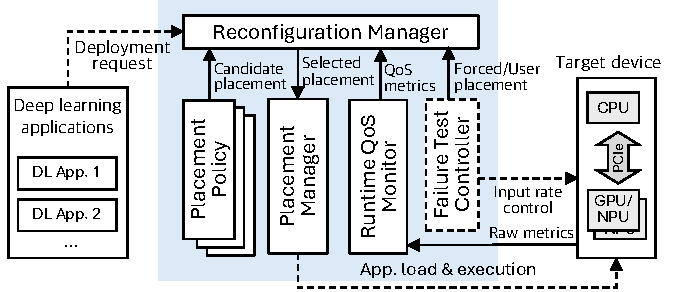
\includegraphics[width=\columnwidth]{architecture.pdf}
\caption{Overview of BoundGuard. The system detects sustained QoS violations and performs validation-driven candidate evaluation to bound the duration of ineffective placements \textcolor{navyblue}{without a system-wide pause}.}
\label{fig:architecture}
\end{figure}

Figure~\ref{fig:architecture} shows the overall architecture of BoundGuard. 
The framework consists of five components: Runtime QoS Monitor, Reconfiguration Manager, Placement Policy, Placement Manager, and Failure Test Controller.
These components collectively enable BoundGuard to treat incorrect placement decisions as transient failures and enforce bounded failure persistence at runtime by evaluating candidate placements under bounded validation windows.

% \noindent\textbf{Runtime QoS Monitor.}
\subsection{Runtime QoS Monitor}
The Runtime QoS Monitor tracks system performance and detects sustained QoS degradation using the violation score $V(t)$ defined in Section~\ref{problem_context}. 
It continuously observes end-to-end latency $\ell_i(t)$ for active applications and computes the windowed violation score over a monitoring interval.
Each application reports per-request latency, including inference time and queue wait time, to a per-application monitoring thread, which maintains running statistics used as $\ell_i(t)$. 
A system-wide timer periodically samples these statistics across all applications to compute the instantaneous violation $v(t)$ and update the sliding-window score $V(t)$.

Using this windowed formulation, the monitor focuses on persistent QoS degradation while filtering transient fluctuations.
Because $\ell_i(t)$ includes queue wait as well as inference time, contention becomes visible to the monitor even when per-request inference latency is unchanged. \textcolor{navyblue}{Transition transients are handled by the window rather than measured through it: a hot-swap perturbs latency for a period short relative to $T$, so it does not by itself move $V(t)$ across the threshold, and reconfiguration triggers are in any case suppressed while a candidate is under validation. Transitions that relocate a background generative model are long enough to interrupt sampling altogether, so they contribute no observations rather than misleading ones.}

The computed $V(t)$ is periodically updated and provided to the Reconfiguration Manager, which triggers reconfiguration when the violation exceeds a predefined threshold.

% \noindent\textbf{Reconfiguration Manager.}
\subsection{Reconfiguration Manager}

The Reconfiguration Manager serves as the central control component for runtime adaptation. 
When sustained QoS degradation is detected (i.e., $V(t) > \epsilon$), indicating an ineffective placement, it initiates recovery by retrieving candidate placements and evaluating them sequentially.
%
Each candidate is treated as a hypothesis and is applied for a bounded validation window, during which the system observes the resulting QoS behavior after a short stabilization period. 
A candidate is retained only if it satisfies the QoS constraint (i.e., $V(t) \le \epsilon$). If not, it is discarded and the system continues evaluating subsequent candidates.

\textcolor{navyblue}{If the candidate budget is exhausted without any candidate being retained---the case in which no QoS-satisfying placement exists---the system does not simply remain on the last placement it happened to try, since the ordering of the candidate list gives no reason to prefer it. Instead it reverts to the best placement observed during the search. We rank the observed candidates by their measured service rate over the validation window rather than by their violation score: the violation score of a later candidate is inflated by the backlog that earlier failed candidates accumulated, which would bias the choice toward whichever candidate was evaluated first, whereas the service rate estimates $\mu_i$ directly and remains meaningful even when the queue is saturated. Candidates that were skipped without evaluation are excluded from this comparison, so reverting can never return the system to a placement already known to be violating.}

Correctness is not assumed from the candidate generation process, but is enforced through runtime validation. 
Candidates are not interpreted as alternative policy decisions, but as placements that must be validated before being accepted.
%
This process is not designed to identify an optimal placement. 
Instead, it enforces bounded failure persistence by ensuring that the system does not remain in any ineffective placement beyond the bounded validation window. 
By limiting the time spent on each candidate, the system prevents prolonged degradation and provides controlled recovery behavior.

To maintain stability, additional reconfiguration triggers are suppressed during validation. 
If no candidate satisfies the QoS constraint, the system continues evaluation with alternative candidates, ensuring that ineffective placements are not retained indefinitely.
%
Importantly, the system does not assume that a QoS-satisfying placement always exists. 
Even when all candidates are ineffective, BoundGuard bounds how long any single placement is held while alternatives remain to be tried, \textcolor{navyblue}{and terminates on the best placement it observed rather than on whichever candidate happened to be last.}

% \noindent\textbf{Placement Policy.}
\subsection{Placement Policy}
\label{sec:placement_policy}
The Placement Policy generates candidate placements that guide runtime adaptation.
Given the current workload and system context, it produces an ordered list of candidate placements, which are evaluated sequentially by the Reconfiguration Manager.
Rather than directly applying a single predicted placement, BoundGuard treats policy outputs as candidates to be validated at runtime.

This design improves robustness under dynamic and partially observable conditions, where prediction errors and interference can lead to ineffective placements.
The policy is not required to produce an optimal placement, as correctness is enforced through runtime validation.
The policy prioritizes candidates that are likely to satisfy QoS constraints. \textcolor{navyblue}{It does not, however, guarantee that the list is diverse. A list ranked by a single predicted score tends to be correlated near its head: placements that share whatever the score rewards occupy consecutive positions, so the alternatives the system tries first may differ from one another far less than the ranking's length suggests. This is a property of the policy rather than of the runtime, but it determines how much the runtime can recover from, and Section~\ref{sec:evaluation} reports a case where it is the binding constraint.}

The Placement Policy is designed as a pluggable component.
In our current implementation, the policy provides a ranked list of candidate placements using a lightweight learned predictor trained on offline profiling data.
Specifically, we use gradient-boosted decision tree models (e.g., XGBoost) to estimate placement performance and guide candidate ranking.
Any method that generates a ranked list of candidate placements can be integrated, enabling the use of different strategies without modifying the runtime adaptation logic.

While our implementation is prediction-based, the ranked-candidate interface does not restrict the class of admissible policies.
Optimization-based methods that natively return a single solution can be adapted with modest effort: the $k$ best solutions encountered during the search can be retained instead of only the incumbent, the problem can be re-solved under perturbed constraints or objectives to obtain diverse alternatives, and previously validated placements can be included as known-good fallbacks.
Moreover, because candidates are retrieved from the policy at recovery time rather than fixed at deployment, the interface permits the list to be regenerated using the current system state, including re-invoking the policy when the available candidates are exhausted.
A conservative fallback placement (e.g., a profiled default configuration) can also be appended to every candidate list, ensuring that the exploration space is never empty.
The framework therefore assumes only that \emph{some} ordered set of alternatives can be produced on demand---a requirement that prediction-based, optimization-based, and rule-based policies can all satisfy.

\subsection{Placement Manager}
\label{sec:placement_manager}
The Placement Manager maintains and applies placements across heterogeneous devices (CPU, GPU, NPU), routing incoming requests to the device where the corresponding model is currently placed.
%
To avoid service disruption, it performs incremental, per-model updates rather than full restarts. 
Given a new placement, only components whose device assignments change are updated, while others continue execution without interruption.

In resource-constrained environments, placement updates must be performed in-place without relying on redundant resources or parallel execution capacity, making safe transitions particularly challenging.
%
For models that require migration, the manager applies a hot-swap transition that overlaps execution across devices, enabling seamless placement updates without interrupting ongoing requests whenever concurrent execution is supported.

\noindent\textbf{Hot-Swap Transition: }
For each model whose device assignment changes, the Placement Manager performs a staged transition that preserves continuous request processing.

First, a new instance is initialized on the target device while the existing instance continues serving requests on the original device. 
This overlapping execution avoids any gap in processing capacity during the transition.
%
Once the new instance becomes ready, request routing is atomically redirected to the new instance. 
From this point, all incoming requests are processed by the new instance, while the previous instance completes processing of any ongoing requests.
%
After all requests already in progress have been completed, the previous instance is terminated.
Because routing is switched atomically and execution overlaps during initialization, the transition avoids both \textcolor{navyblue}{transition-induced} request loss and duplication.

This design ensures that there is no interval during which the system is unable to process requests. 
\textcolor{navyblue}{As a result, a placement update interrupts only the application instances it actually moves, avoiding the system-wide pause that stop-and-restart incurs.}

\noindent\textbf{Heterogeneous Execution Considerations: }
While the same transition mechanism is applied across all devices, execution constraints vary by device type. 
CPU and GPU workers support concurrent execution, allowing overlapping transitions as described above.

In contrast, some accelerators (e.g., NPUs) do not support concurrent execution on the same device. 
In such cases, transitions are performed in a controlled manner with temporary request buffering, which preserves continuity and limits the impact to a transient latency increase. \textcolor{navyblue}{This buffer is finite; under sustained overload it may overflow, in which case excess requests are dropped and counted as deadline misses (Section~\ref{subsec:metrics}), distinct from the switching mechanism itself, which incurs no request loss.}
%
Despite these differences, the transition semantics remain consistent. New instances are activated only after initialization, and previous instances complete ongoing requests before termination whenever possible. 
This ensures reliable and continuous execution across heterogeneous devices.

%This abstraction ensures that device-specific constraints do not affect the correctness or continuity of placement transitions.


% \noindent\textbf{Failure Test Controller.}
\subsection{Failure Test Controller}
\label{sec:failure_test_controller}
The Failure Test Controller is an evaluation-only component used to systematically generate controlled runtime conditions that induce QoS degradation. It introduces controlled perturbations, such as ineffective initial placements, input rate changes, and background interference, to trigger sustained QoS violations.
%
These conditions are designed to expose placement failures arising from resource contention, workload dynamics, and prediction errors. 
By triggering controlled degradation scenarios, the controller enables systematic evaluation of detection latency, recovery behavior, and failure impact.

Importantly, the controller operates entirely outside the runtime control loop. It interacts with the system only through external inputs, including workload configuration and resource usage, without modifying or bypassing any adaptation mechanism. 
This ensures that evaluation results reflect the behavior of the unmodified system under realistic runtime conditions.

\section{Experimental Evaluation}
\label{sec:evaluation}

We evaluate the effectiveness, robustness, and generality of BoundGuard under diverse workload conditions.
To guide our evaluation, we address the following questions:

\begin{itemize}
\item[\textbf{Q1}] How do incremental reconfiguration mechanisms affect failure impact and recovery behavior?
\item[\textbf{Q2}] Can validation-driven adaptation recover reliably under dynamic workload changes?
\item[\textbf{Q3}] Does validation improve robustness to incorrect ML-based placement decisions?
\item[\textbf{Q4}] Can BoundGuard provide bounded behavior when candidate placements fail to satisfy QoS within the validation window?
\item[\textbf{Q5}] Does BoundGuard generalize to constrained heterogeneous platforms (e.g., CPU--NPU)?

% \item[\textbf{Q6}] Sensitivity to candidate quality.
\end{itemize}


\subsection{Experimental Setup}

\subsubsection{Hardware Platforms}

\noindent\textbf{\newline CPU--GPU platform.}
We evaluate our framework on a desktop system with an Intel Core i7-13700K CPU and an NVIDIA GeForce RTX 5090 GPU (32\,GB), connected via PCIe Gen5~$\times$16. 
This platform exhibits rich host--device interference and serves as the primary evaluation environment.

\noindent\textbf{CPU--NPU platform (constrained accelerator).}
\textcolor{navyblue}{To assess robustness under constrained accelerators, we additionally evaluate on a CPU--NPU system with an Intel Core i7-13700K CPU and a single PCIe-attached Mobilint MLA100 (ARIES) NPU~\cite{oh2025optimizing}, driven by the vendor \texttt{qbruntime} stack. The NPU exposes eight cores organized as two clusters of four local cores, and models are compiled ahead of time into fixed \texttt{uint8} device binaries. Its constraints differ in kind from those of a GPU: models must be quantized and compiled offline, operator support is limited, and the per-model core assignment acts as a placement hint rather than an exclusive reservation, with the runtime scheduler time-sharing the device among co-resident models. Multiple models can therefore remain resident simultaneously, and the binding limit on concurrency is device memory (16\,GB) rather than the core count.}


\subsubsection{Benchmark Models and Workloads}

%%---- 앱실론: 1.0으로 설정
%%----"We set $L_{SLO,i} = 5 \cdot \text{latency}_i$ to allow sufficient headroom for inter-model contention observed in heterogeneous concurrent execution."  
\begin{table}
\centering
\caption{Benchmark models for CPU--GPU evaluation. \textcolor{navyblue}{Vision latencies are isolated end-to-end pipeline times (median of 300 runs, measured after a GPU pre-warm-up so that first-session initialization cost is not attributed to any single model); the generative models report end-to-end latency for 64-token generation. $L_{SLO}$ is applied only to the foreground (vision) models, so it is marked ``--'' for the background LLM/VLM. $^{\dagger}$Qwen2-VL was measured with the conv3d vision encoder falling back to a non-cuDNN path due to a cuDNN version mismatch on our system, and may be faster with a matched cuDNN.}}
\label{tab:gpu_models}
\begin{tabular}{@{}l l r r r@{}}
\hline
\multirow{2}{*}{\textbf{Model}} & \multirow{2}{*}{\textbf{Category}} & \textbf{Size} & \textbf{Latency} & \textbf{$L_{SLO}$} \\
 &  & \textbf{(MB)} & \textbf{(ms)} & \textbf{(ms)} \\
\hline
YOLO11n & Detection & \textcolor{navyblue}{11} & \textcolor{navyblue}{5.07} & \textcolor{navyblue}{25.4} \\
YOLO11s & Detection & \textcolor{navyblue}{37} & \textcolor{navyblue}{6.19} & \textcolor{navyblue}{31.0} \\
YOLO11m & Detection & \textcolor{navyblue}{77} & \textcolor{navyblue}{8.36} & \textcolor{navyblue}{41.8} \\
YOLO11l & Detection & \textcolor{navyblue}{98} & \textcolor{navyblue}{10.31} & \textcolor{navyblue}{51.6} \\
YOLO11x & Detection & \textcolor{navyblue}{218} & \textcolor{navyblue}{13.07} & \textcolor{navyblue}{65.4} \\
ResNet50 & CNN (classification) & \textcolor{navyblue}{98} & \textcolor{navyblue}{2.24} & \textcolor{navyblue}{11.2} \\
MobileNet-v2 & Lightweight CNN & \textcolor{navyblue}{14} & \textcolor{navyblue}{1.28} & \textcolor{navyblue}{6.4} \\
LLaMA-1B & LLM (Transformer) & \textcolor{navyblue}{2{,}357} & \textcolor{navyblue}{302.0} & \textcolor{navyblue}{--} \\
Qwen2-VL & VLM (vision--language) & \textcolor{navyblue}{4{,}213} & \textcolor{navyblue}{840.0$^{\dagger}$} & \textcolor{navyblue}{--} \\
\hline
\end{tabular}
\end{table}


\noindent\textbf{\newline CPU--GPU workloads.}
We construct multi-application workloads using diverse model types, including CNNs, detection models, and transformer-based language models (Table~\ref{tab:gpu_models}). 
%The reported latency values correspond to end-to-end per-request latency under isolated execution, including both model execution and input/output processing overhead.
The reported latency values correspond to end-to-end per-request latency under isolated execution, including both model execution and input/output processing overhead.
We set $L_{SLO,i} = 5 \cdot \text{latency}_i$ to provide sufficient headroom for inter-model contention observed in concurrent heterogeneous execution.

\textcolor{navyblue}{We designate three vision models (YOLO11s~\cite{yolo11}, ResNet50~\cite{resnet}, and MobileNet-v2~\cite{mobilenetv2}) as foreground workloads, whose latency is monitored to compute the QoS violation score $V(t)$. A generative model runs alongside them as a fourth application instance. Its own latency is not monitored---it is background load, present to create contention---but it is a placement target like the others, so the runtime may move it between the accelerator and the CPU. A workload of four applications over two devices therefore yields a candidate space of sixteen placements. The remaining models (YOLO11m, YOLO11n/l/x, and whichever generative model is not in use) constitute a pool of additional background loads; each experiment states which of them are active.}
\textcolor{navyblue}{This composition is deliberate. We also ran a variant with four vision applications in the foreground and found that it does not exercise the mechanism under study. The reason is that the binding resource is the CPU-side pipeline stage rather than the accelerator: with four vision applications the CPU has no headroom left, so relocating the generative model onto it makes matters worse rather than better. Measured at a load high enough to induce violation, the placement our policy ranks as the recovery reaches $V(t)=5.2$ against $3.4$ for the top-ranked placement---the intended remedy is the worse of the two. With three vision applications the CPU retains enough headroom for the relocation to pay off, and the same placement recovers. We report the three-model composition because it is the one in which placement is the binding decision.}
Foreground models are used to compute the QoS violation score, while background models are introduced to generate resource contention and interference without directly affecting the QoS metric. This separation allows us to isolate the impact of interference from workload dynamics, which are evaluated separately through input rate variation.

By combining models with different resource demands, we capture both compute-bound and memory-bound interference patterns. 
We construct workloads with up to nine concurrent application instances to evaluate system behavior under increasing contention.



\noindent\textbf{Model availability across platforms.}
Model availability is platform-dependent due to accelerator constraints. On the CPU--GPU platform, all models are executed using standard ONNX runtimes. 
On the CPU--NPU platform, only a subset of models is supported due to limited operator support and deployment constraints. \textcolor{navyblue}{Vision models are compiled to the NPU (\texttt{.mxq}) ahead of time; models outside the supported set fall back to the CPU backend.}


\noindent\textbf{CPU--NPU workloads.}
On the CPU--NPU platform, we construct workloads with four concurrent application instances, \textcolor{navyblue}{composed as above: three vision applications whose latency is monitored, and a generative model that contributes contention without entering the QoS score while remaining a placement target.}
This reflects the limited capacity and reduced co-location flexibility of NPUs, where each placement decision has a stronger impact on overall performance.
%
\textcolor{navyblue}{We draw base models from our vision set (e.g., ResNet50 and YOLO11) and, where supported, generate NPU-executable variants via quantization and compilation.
Because co-residency on the MLA100 is bounded by device memory rather than by a single-model restriction, several models can be held resident concurrently and are time-shared by the runtime scheduler; each application instance is assigned either to the NPU or to the CPU backend during runtime reconfiguration.}

To induce contention, we vary input rates dynamically. 
This setup evaluates whether BoundGuard can maintain bounded recovery behavior under restricted execution environments with limited placement flexibility.



\subsubsection{Baselines and Incremental Mechanisms}

We compare four execution modes that incrementally incorporate the key mechanisms of runtime placement adaptation.
This design allows us to isolate the contribution of each mechanism to failure handling.

\noindent\textbf{Static placement.}
Uses a fixed configuration without runtime adaptation. 
The system does not perform reconfiguration after deployment.

\noindent\textbf{Stop-and-restart.}
Performs reactive reconfiguration by selecting a new placement using a policy and redeploying it upon performance degradation. 
It applies a single placement decision at a time and restarts execution during each transition.

\noindent\textbf{Adaptive hot-swap.}
Performs runtime reconfiguration using a placement policy, applying a single placement decision at a time while preserving execution continuity through hot-swap transitions. 
Placements are applied without validation.
\textcolor{navyblue}{Concretely, it re-invokes the policy on each detected violation and applies whatever placement is returned; it neither observes a candidate before judging it nor descends a ranked list. In the terms of Section~\ref{problem_context} it is therefore the corner of the $2\times2$ design in which both dwell and progress are absent, and it is the closest baseline to the unconstrained reactive loop discussed there. Q6 completes the remaining two corners.}

\noindent\textbf{BoundGuard.}
Performs validation-driven runtime adaptation by evaluating candidate placements based on QoS feedback. 
Given a set of candidates from a placement policy, each is applied for a bounded validation window and evaluated using $V(t)$. 
Candidates are retained only if they satisfy the QoS constraint, while others are replaced by alternative candidates through iterative evaluation.

\textcolor{navyblue}{\subsubsection{Evaluation Metrics}
\label{subsec:metrics}
The violation score $V(t)$ defined in Section~\ref{problem_context} drives the control loop, whereas the reported reliability outcome is measured at the request level. Each request of application instance $i$ carries the deadline $L_{SLO,i}$; a request is a \emph{deadline miss} if its end-to-end response time exceeds $L_{SLO,i}$ or if it is dropped before completion. The \emph{deadline miss rate} is the fraction of arrived requests that are deadline misses,
\begin{equation}
\mathrm{miss\ rate} = \frac{N_{\mathrm{late}} + N_{\mathrm{drop}}}{N_{\mathrm{arrived}}},
\end{equation}
where $N_{\mathrm{late}}$ counts requests completing after their deadline and $N_{\mathrm{drop}}$ counts requests dropped on buffer overflow. \textcolor{navyblue}{Both late completions and drops are counted as misses; we additionally report their split, as the share of drops within the miss rate reflects how severely condition~C3 is violated.} Requests are admitted into a finite buffer of capacity $B$; when sustained overload drives the backlog beyond $B$ (a violation of condition~C3 in Section~\ref{problem_context}), excess requests are dropped and, as above, counted as deadline misses rather than silently excluded, so buffer overflow degrades the reported reliability rather than flattering it. \textcolor{navyblue}{We size $B$ relative to the worst-case backlog predicted by the fluid model of Section~\ref{problem_context}, $Q_{\max} \approx T + N_{cand}(T_v+\delta)$ times the overload rate, and sweep $B = \beta_B \cdot Q_{\max}$ across three regimes, $\beta_B \in \{1.5,\ 1.0,\ 0.5\}$, corresponding to slack (no drops, so the fluid model can be validated against the measured backlog trajectory), the boundary, and a tight buffer that deliberately induces drops. Equivalently, $B$ is expressed as a time horizon of peak arrivals, $B = \lceil \lambda_{\mathrm{peak}} \cdot \tau_B \rceil$, so that the setting is interpretable independently of hardware throughput.} In addition to the aggregate miss rate, we report the $p99$ and $p999$ tail response times over the adaptation interval, since the transient severity of recovery is hidden by a mean-based metric. Throughout, $V(t)$ is the detection signal that triggers reconfiguration, while the deadline miss rate and tail latency are the outcome metrics used to compare methods.}

\subsubsection{Evaluation Parameters}
QoS violation is computed at a sampling interval of \textcolor{navyblue}{$\Delta = 0.2$\,s} with a monitoring window of $T = 3$\,s. 
Unless otherwise stated, we use $T_v = 3$\,s for candidate validation and $\epsilon = 1.0$ as the violation threshold throughout the experiments.
This threshold corresponds to the point where the average latency exceeds the SLO by 100\%.
\textcolor{navyblue}{We selected $\Delta$ empirically, subject to the ordering constraint $T_v \ge T > \Delta$: sweeping $\Delta$ offline over recorded per-request traces, we chose the shortest interval that produced no spurious threshold crossings during feasible operation while keeping the detection lag well below $T$. Because $V(t)$ averages $v(\tau)$ over $T$, the measured recovery time cannot fall below $T$ regardless of how quickly the system itself recovers; this floor is a property of the monitor, not of the placement.}

\subsection{Results and Analysis}
\noindent\textbf{Q1: How do incremental reconfiguration mechanisms affect failure impact and recovery behavior?}

We first examine how the progressive addition of reconfiguration, seamless switching, and validation affects system behavior under harmful runtime placements.
These mechanisms represent four distinct failure-handling strategies.
Static leads to persistent and uncontrolled degradation due to the absence of corrective action.
Stop-and-restart bounds recovery but introduces service disruption.
Adaptive hot-swap preserves execution continuity, but may propagate incorrect decisions by committing to unvalidated placements.
In contrast, BoundGuard achieves both continuity and bounded recovery through validation-driven candidate evaluation, which ensures that no ineffective placement persists beyond a bounded duration.

\begin{figure}[tb]
\centering
\includegraphics[width=\columnwidth]{bounded_recovery_analysis.pdf}
\caption{\textcolor{navyblue}{Recovery latency per scenario, split into the lead (violation onset until the first candidate is in service), the search (until the admitted candidate is in service), and the drain (until $V(t)\le\epsilon$), against the envelope instantiated from each run's own measured $k$ and $\delta$. The lead is dominated by a fixed wait our harness imposes before the first candidate may be applied, and is separated for that reason. Every run that recovers stays inside its envelope. The infeasible-candidate scenario is shown apart: it does not recover, so it has no admitted candidate and no drain, and its bar is a terminal violation rather than a recovery latency.}}
\label{fig:bounded_recovery}
\end{figure}

We measure the recovery latency $T_{recovery}$ from the onset of failure-inducing conditions to the point where the system returns to a stable state ($V(t) \le \epsilon$).
Following Section~\ref{problem_context}, we decompose:
\begin{equation}
T_{recovery} = T_{detect} + T_{post}.
\end{equation}
where $T_{post} = T_{valid} + T_{stable}$ groups the validation and stabilization terms of Eq.~(\ref{eq:recovery_decomposition}).

We evaluate this behavior across diverse contention scenarios using four foreground models.
Figure~\ref{fig:bounded_recovery} shows the breakdown of recovery latency.

To relate analytical guarantees with observed behavior, we instantiate the recovery bound under our configuration.
With $T=3$\,s, $T_v=3$\,s, $N_{cand}=5$, $\delta \approx 1$\,s, and $T_{stable} \approx 10$\,s:
\begin{equation}
T_{recovery} \le 3 + 5 \cdot (3 + 1) + 10 = 33\,\text{s}.
\end{equation}

\textcolor{navyblue}{Recovery completes in $30.4\pm0.5$\,s on CPU--GPU and $27.2\pm0.4$\,s on CPU--NPU, in both cases within the envelope instantiated from the measured transitions of each run. Both are measured from the first violation. A large share of each is the lead $L$ of Eq.~(\ref{eq:recovery_bound})---$9.0$\,s on the GPU and $22.4$\,s on the NPU---during which the controller cannot yet apply a candidate; on the NPU $9.6$\,s of that precedes the controller being enabled at all, because the stable phase there is already violating. Detection is bounded by the monitoring window by construction and was stable across scenarios; we therefore report the post-detection phases, which are what the placement policy influences.}

The gap between the analytical bound and observed latency arises because the bound assumes worst-case exploration of all candidates.
In practice, the system converges within fewer validation steps than the maximum allowed ($N_{cand}=5$), resulting in substantially lower latency.
This confirms that the bound is conservative, providing a worst-case guarantee rather than a tight estimate.

Overall, recovery latency is governed by bounded validation rather than prolonged persistence of incorrect placements.
This bounded recovery behavior provides the foundation for controlling failure impact, which we analyze in Q1.3.

\begin{figure}[t]
\centering
\includegraphics[width=\columnwidth]{runtime_overhead.pdf}
\caption{\textcolor{navyblue}{Steady-state cost relative to Static, which performs no monitoring. Bars whose magnitude falls inside the run-to-run spread are marked as such; the CPU difference changes sign between the two platforms.}}
\label{fig:runtime_overhead}
\end{figure}

\vspace{0.5em}
\noindent\textbf{Q1.1: \textcolor{navyblue}{Steady-state overhead and transition cost.}}

{\color{navyblue}%
We measure what the mechanism costs in two situations: when nothing is happening, and when a placement actually changes.

\emph{Steady state.} We hold the workload in a feasible state throughout ($V(t)=0$, no reconfiguration triggered) and compare against Static, which does no monitoring at all. Each configuration is repeated three times; Figure~\ref{fig:runtime_overhead} reports the mean and standard deviation. Throughput is identical to the arrival rate in every arm on both platforms ($12.1$\,fps, no dropped frames), so the comparison rests on latency and CPU occupancy. Per-view inference latency is $2.4$--$2.6$\,ms on the GPU and $2.8$--$2.9$\,ms on the NPU, with the arms ordered differently on the two platforms. Executor CPU occupancy is $16.5$--$16.7\%$ on the GPU and $17.4$--$17.7\%$ on the NPU.

The monitoring cost is not resolvable at this scale, and the sign of the difference is not even consistent: relative to Static, BoundGuard uses $0.18$ percentage points \emph{less} CPU on the GPU and $0.12$ points more on the NPU, both within the run-to-run spread. The correct statement is therefore that we observe no steady-state cost, not that we measure a small one. We also note what this experiment can and cannot compare. Static differs from the other two arms in doing no monitoring, and that is the contrast the numbers speak to. Adaptive hot-swap and BoundGuard, by contrast, execute the same code path when nothing is happening---everything BoundGuard adds is transition-time behavior, and there are no transitions here---so their agreement is a consistency check rather than a finding.

\emph{Transition.} The switching mechanism is supposed to move a placement without losing or duplicating requests. We test this directly, using a buffer large enough ($B=2000$) that overflow drops cannot be confused with switching losses, and a schedule that performs several hot-swaps in sequence. For every view we account for each admitted request: those completed, those dropped, and those still queued at the end. The accounting balances to within one to three in-flight frames on both platforms, and no request is dropped at any transition---the inherited backlog, several hundred frames deep, is carried over to the new worker in full. No request is completed twice.

Service continuity is more nuanced than a single yes or no, and worth stating precisely. Views whose placement does not change continue to serve throughout the transition; their largest gap between consecutive completions ($0.15$--$0.21$\,s) is the normal inter-frame interval. A view that is migrated pauses for about $1.0$\,s while its replacement worker initializes. Stop-and-restart, by contrast, halts \emph{every} view simultaneously for $1.5$--$2.2$\,s, since it tears down and rebuilds the whole deployment. The advantage of in-place switching is therefore that the interruption is confined to the applications actually being moved, and is roughly half as long---not that it disappears.}

\vspace{0.5em}
\noindent\textbf{Q1.2: Detection parameter sensitivity}

\begin{figure}[t]
\centering
\includegraphics[width=\columnwidth]{detection_sensitivity.pdf}
\caption{Sensitivity to detection parameters $(T, \epsilon)$. Detection latency increases with the monitoring window and remains bounded by it, while recovery behavior remains stable.}
\label{fig:detection_sensitivity}
\end{figure}

{\color{navyblue}%
Detection is governed by two parameters: the monitoring window $T$ over which $v(\tau)$ is averaged, and the threshold $\epsilon$. We sweep $T \in \{1,3,5\}$\,s against $\epsilon \in \{0.5, 1.0, 2.0\}$. \textcolor{navyblue}{Only the first two windows are admissible designs: the ordering constraint $T_v \ge T > \Delta$ of Section~\ref{problem_context} excludes $T=5$\,s at our $T_v=3$\,s, because a validation window shorter than the monitoring window would judge a candidate on an average that still contains pre-transition samples. We include it to show the trend continuing rather than as a setting one could adopt.} \textcolor{navyblue}{The sweep is computed offline by re-windowing the recorded $v(\tau)$ series of the $25$ misprediction runs of Q3 and Q6, so every setting sees identical input and the input is the same workload the rest of this section reports.}

\textcolor{navyblue}{Figure~\ref{fig:detection_sensitivity} reports four quantities. No setting produces a false detection: the false-positive count is zero across the whole grid, including the shortest window. Detection lag tracks the window almost exactly---$0.6$\,s at $T=1$, $2.0$\,s at $T=3$, $4.0$\,s at $T=5$---and that lag propagates: recovery latency rises with it, from $18.0\pm5.3$\,s to $21.8\pm6.0$\,s across the same range, while cumulative violation is flat to within its spread.}

Our configuration ($T=3$\,s, $\epsilon=1.0$) sits in the conservative corner of this space. \textcolor{navyblue}{The sweep does not support it, and we say so directly: among the admissible windows, $T=1$ dominates it on this data---detecting sooner ($0.6$\,s against $2.0$), recovering sooner ($18.0$\,s against $20.2$), and producing no false detections either. What the sweep cannot tell us is what $T=3$ is buying, because these traces contain no transient spike for a longer window to absorb. The honest statement is therefore not that $T=3$ is justified but that the cost of $T=1$ was not observed here; a workload with brief latency excursions would be needed to test the difference, and we did not construct one. We retain $T=3$ because it is the setting under which every other experiment in this section was run.}

\vspace{0.5em}
\noindent\textbf{Q1.3: Failure persistence and cumulative impact.}

Building on Q1, we analyze failure impact using two complementary metrics derived from $V(t)$: failure persistence and cumulative QoS violation. 
Failure persistence measures the duration for which $V(t) > \epsilon$, while cumulative violation captures the time-integrated excess above the threshold.

\begin{figure}[t]
  \centering
  \includegraphics[width=\columnwidth]{q13_failure_persistence.pdf}
  \caption{\textcolor{navyblue}{Recovery outcome (left) and, for the methods that recover, how long the violation lasts (right). Static never returns below $\epsilon$ on either platform, so it has no persistence to report and does not appear in the right panel; its terminal violation is shown on the left instead.}}
  \label{fig:q13-persistence}
\end{figure}

\begin{figure}[t]
  \centering
  \includegraphics[width=\columnwidth]{q13_cumulative_violation.pdf}
  \caption{\textcolor{navyblue}{Cumulative QoS violation $\int V(t)\,dt$ over the same runs.}}
  \label{fig:q13-cumulative}
\end{figure}

{\color{navyblue}%
Figures~\ref{fig:q13-persistence} and~\ref{fig:q13-cumulative} report both metrics for the four methods on both platforms. Each configuration is repeated five times. Static is the outlier: on neither platform does it return below $\epsilon$ within the observation window, ending at $V(t)\approx13.8$, so its failure persistence is censored by the window length ($94$\,s) rather than measured. What we can report of it is the integrated quantity: it accumulates $1279\pm1$ and $1295\pm7$ units of violation. The three methods that reconfigure recover in every run and land close to one another---persistence of $13.2$--$15.2$\,s and cumulative violation of $147$--$162$---and their error bars overlap, so we cannot separate them here. On the integrated metric they are roughly eight times lower than Static ($8.3\times$ on the GPU, $8.4\times$ on the NPU), computed over a window fixed at $94$\,s for every method so that the ratio is not an artifact of unequal observation lengths.

We do not read the small differences among stop-and-restart, Adaptive hot-swap, and BoundGuard as meaningful; across five runs they fall inside one another's spread. \textcolor{navyblue}{The reason is visible in the search: the recovering placement is the predictor's first choice here ($k=1$), so there is no candidate list to descend and BoundGuard's search reduces to applying that one placement. Its measured search of $10.8$\,s is the harness lead $L$ and nothing else---the mechanism contributes no additional time. Separation between the methods appears only when the first choice is wrong, which is Q3.} In this workload the predictor's choice is correct, so all three converge on the same placement and differ only in how they reach it; Q1.5 makes the same observation with request-level metrics. \textcolor{navyblue}{This equivalence should not be read as evidence that validation is dispensable under correct prediction. It holds because a policy re-invoked under unchanged conditions returns the same feasible placement, so Adaptive hot-swap converges after a single transition and has no opportunity to misbehave. Q6 shows that a variant which retains candidate traversal but drops the dwell window breaks even in this regime---recovering in only two runs of five, and making fifteen transitions where the others make six---which locates the safety of Adaptive hot-swap in the brevity of its search rather than in the sufficiency of unvalidated reconfiguration.} In particular we do not treat stop-and-restart's low persistence as an artifact of its downtime suppressing latency measurements: we checked the traces for that signature---intervals where $V(t)$ falls below $\epsilon$ while the backlog is still large or throughput has collapsed---and found none. Its restart completes quickly enough that the first post-restart sample already shows the system serving, and its recovery here is genuine.

What this experiment establishes is the weaker but necessary claim that bounded validation does bound the impact. The distinction among the adaptive methods emerges only when the prediction is wrong, which is the subject of Q3.}

{\color{navyblue}%
\vspace{0.5em}
\noindent\textbf{Q1.4: Does the fluid recovery model match measured queue dynamics?}

Section~\ref{problem_context} models the stabilization phase with a deterministic fluid approximation, in which the backlog accumulates at rate $\lambda-\mu_i$ during failed validations and drains at rate $\mu^{\ast}-\lambda$ once a QoS-satisfying placement is accepted, so that $T_{stable}=Q(k)/(\mu^{\ast}(\lambda)-\lambda)$ diverges as the offered load approaches what the accepted placement can serve. We validate this model directly by logging per-window queue lengths and reconstructing the accumulation and drain slopes on both platforms, sweeping the arrival rate relative to the service rate ($\lambda=0.70,0.90,0.95\times\mu^{\ast}$).

\begin{figure*}[t]
\centering
\includegraphics[width=0.92\textwidth]{c3_fluid_validation.pdf}
\caption{\textcolor{navyblue}{Fluid recovery model against measurement over an arrival-rate sweep on both platforms, with no dropped frames anywhere in the sweep so that the queue is conserved. Accumulation matches the predicted slope closely. Drainage matches in shape---the slope scales with $\lambda$ as predicted and falls toward zero as the load rises---but not in magnitude under any single service rate; the rate that fits differs from one measured at a light probe load. The highest GPU load is marked as having no drain rather than a large one: there the effective rate leaves no spare capacity, so the backlog does not drain and the stabilization time is undefined. The stabilization times annotated in (c) are extrapolated from the measured slope; only the lowest CPU--NPU load actually emptied its queue within the observation window.}}
\label{fig:fluid_validation}
\end{figure*}

The sweep separates the model's two halves, and they do not fare the same. Accumulation is reproduced tightly: the measured slope follows $\lambda-\mu_{cpu}$ to within $0.2\%$ in all eighteen cells, and no frames are dropped anywhere in the sweep, so the queue is conserved and the fluid description applies. Drainage is where the model is only half right. Its functional form holds---regressing the measured drain slope against $\lambda$ gives $1.007$ on the GPU and $1.083$ on the NPU against a predicted $1.0$, and the slope falls monotonically toward zero as the load rises on both platforms---but no single constant $\mu^{\ast}$ reproduces the magnitudes. Against the three candidate rates we registered in advance, none matched to our stated tolerance in any of the eighteen cells.

The reason is the one Eq.~(\ref{eq:tstable}) now names. Inverting the measurements for the service rate that would fit gives a value that is stable within each load ($\pm0.15$\,fps on the GPU, $\pm0.79$ on the NPU) but differs from the anchor measured at a light probe load by $-6.8\%$ and $+12.5\%$ respectively. The end-to-end pipeline rate is a real quantity---the earlier observation that it is roughly half the raw inference rate is reproduced, with saturation at $79$ and $65$\,fps bracketing the effective drain rates of $113$ and $97$ against inference alone at $144$ and $231$---but it is not a single number. Which stage saturates, and therefore what the placement can actually deliver, shifts with the load it is asked to carry.

The consequence is concrete rather than theoretical, and it appears at the top of the sweep. At what the anchor rate calls $0.95\,\mu^{\ast}$---nominally five percent of spare capacity---the ratio computed from the effective rate is $1.02$, so there is no spare capacity at all and the backlog never drains. We report no stabilization time for that cell because none exists: the quantity is undefined, not large. A practitioner sizing headroom from a lightly loaded measurement would have expected recovery there and would not have got it. Elsewhere in the sweep we report stabilization times extrapolated from the measured drain slope rather than observed to completion---only the lowest load we tried emptied its queue inside the observation window---so these are projections of the fitted dynamics, not timings of a recovery we watched finish.}

{\color{navyblue}%
\vspace{0.5em}
\noindent\textbf{Q1.5: How do the methods compare on request-level deadline misses and tail latency?}

We now report the request-level outcome metrics of Section~\ref{subsec:metrics}. We take the $p99$/$p999$ tail response times as the primary quantity and the deadline miss rate (late completions plus drops, over arrivals) as a secondary, diagnostic one; the reason for that ordering is the first observation below. To exercise the drop path, we use the tight-buffer, high-load regime ($\beta_B=0.5$, $\lambda=0.9\,\mu^{\ast}$), which deliberately drives the backlog past the buffer capacity; the absolute miss rates are therefore high by construction, and the quantity of interest is the \emph{relative} behavior across methods rather than the absolute values. Table~\ref{tab:b2} and Figure~\ref{fig:b2} summarize the results on both platforms.

\begin{table}[t]
\centering
\caption{\textcolor{navyblue}{Tail response time and deadline miss rate} under the drop-inducing stress regime ($\beta_B=0.5$, total arrival rate $0.9\,\mu^{\ast}$ divided across the three foreground models). ``drop:late'' is the composition of misses. \textcolor{navyblue}{Deadlines are $15$\,ms uniformly. Both metrics separate the methods here, so we report both; the drop:late column is included because the miss rate alone conflates two different outcomes and the methods differ in which one they produce. All methods are run for a matched wall-clock duration so that the backlog they must service is comparable.}}
\label{tab:b2}
\begin{tabular}{@{}l l r r r r@{}}
\hline
\textbf{Plat.} & \textbf{Method} & \textbf{$p99$} & \textbf{$p999$} & \textbf{Miss} & \textbf{drop:late} \\
\hline
GPU & Static & 33.7\,s & 37.5\,s & 63\% & 65:35 \\
GPU & Stop-restart & 10.1\,s & 10.8\,s & 20\% & 0:100 \\
GPU & Adaptive & 7.6\,s & 8.3\,s & 19\% & 9:91 \\
GPU & BoundGuard & 7.4\,s & 8.2\,s & 19\% & 8:92 \\
\hline
NPU & Static & 32.5\,s & 33.1\,s & 63\% & 54:46 \\
NPU & Stop-restart & 9.5\,s & 10.4\,s & 20\% & 0:100 \\
NPU & Adaptive & 6.8\,s & 7.6\,s & 18\% & 6:94 \\
NPU & BoundGuard & 7.0\,s & 7.8\,s & 19\% & 7:93 \\
\hline
\end{tabular}
\end{table}

\begin{figure*}[t]
\centering
\includegraphics[width=0.86\textwidth]{b2_buffer_sweep.pdf}
\caption{Buffer sweep ($\beta_B\in\{0.5,1.0,1.5\}$): $p99$ end-to-end latency (top) and dropped frames (bottom) on both platforms. The ordering of methods is stable across buffer sizes; the buffer changes only whether excess arrivals surface as drops or as late completions.}
\label{fig:b2}
\end{figure*}

Two observations follow, and both are stable across the buffer sweep of Figure~\ref{fig:b2}. First, enlarging the buffer does not improve deadline attainment so much as change how it is missed. On the GPU, Static's dropped frames fall from $1979$ to $958$ as $\beta_B$ goes from $0.5$ to $1.5$, but its miss rate falls only from $63\%$ to $53\%$ and its tail is flat to within $0.4\%$: the frames the larger buffer retains are admitted only to complete seconds late. This inverts the intuition that slack helps. It also shows that the buffer cannot substitute for a correct placement---Static reaches capacity at every buffer size we tried, because a CPU-only placement cannot service the arrival rate at all, and no amount of queueing changes that.

Second, both metrics separate the methods, and they draw the same line: the primary division is between reconfiguring and staying put. Static misses $63\%$ of deadlines and waits $33.7$\,s at the $99$th percentile; every method that changes the placement misses about $19\%$ and waits $6.8$--$10.1$\,s. That is a factor of $3.3$--$4.7$ on the tail and of more than three on the miss rate, and it holds at every buffer size on both platforms.

Within the reconfiguring group a second, smaller division appears, and it is the one this paper's switching mechanism is about. Stop-and-restart reaches $10.1$\,s at the $99$th percentile where the two in-place methods reach $7.4$--$7.6$\,s---a $26\%$ tail reduction for avoiding the halt, on essentially identical miss rates. The composition column shows why: stop-and-restart drops nothing at all ($0{:}100$) because it admits no frames while it is down, so every affected request arrives late instead. The in-place methods drop a small fraction ($8{:}92$) and finish the rest sooner. Neither outcome is strictly better in the abstract---an early drop and a late completion are different failures---but on the tail, which is the quantity a latency SLO is written against, avoiding the halt is worth about a quarter.

Within that reconfiguring group, the comparison that matters most for this paper is between BoundGuard and Adaptive hot-swap, and on these metrics they are indistinguishable: their $p99$ differs by at most $3\%$ in every swept cell, in one direction on the GPU and the other on the NPU. This is the expected outcome, since the predictor's top-ranked placement is feasible in this workload, so validation admits it immediately and BoundGuard reduces to a single hot-swap. The purpose of this experiment is therefore to establish the absence of a penalty---bounding failure persistence costs nothing when the prediction is already correct. BoundGuard's distinctive behavior appears only when the prediction is wrong, which we examine next in Q3.}

\vspace{0.5em}
\noindent\textbf{Q2: Can validation-driven adaptation recover reliably under dynamic workload changes?}

We evaluate whether validation-driven adaptation can maintain stable performance under dynamic workload changes, where runtime conditions deviate from the initial placement.
%
To induce workload shifts, we increase input rates during execution, pushing the system beyond the capacity of the initial CPU-based placement.

{\color{navyblue}%
\textcolor{navyblue}{This scenario and the prediction-match control of Q6 are the same configuration---the same three foreground models, the same arrival rate, no background load---so we report them together. Before the increase both methods operate with negligible violation. Once the rate rises the CPU-resident placement saturates and $V(t)$ climbs past the threshold. Static stays there for the remainder of the run and never recovers. Every method that reconfigures returns below $\epsilon$ in all five runs, and they are not distinguishable from one another in how long it takes: $13.0$--$13.8$\,s across BoundGuard, Adaptive hot-swap, and the two progress-free variants. The one exception is the variant that removes the dwell window, which recovers in only two runs of five; we return to it in Q6.}

This is the case in which the predictor is right---the offload placement it ranks first is in fact feasible---so what is exercised here is the detection and switching path rather than the search. The candidate is admitted on its first validation and the system converges without evaluating alternatives; the contrasting case, in which the top-ranked placement is not feasible, is the subject of Q3. The workload here is vision-only, with no generative background; interference from a co-resident LLM is exercised in Q3 and Q5.}

\vspace{0.5em}
\noindent\textbf{Q3: Does validation improve robustness to incorrect ML-based placement decisions?}

{\color{navyblue}%
We evaluate the robustness of BoundGuard when the learned predictor selects an ineffective placement. Rather than injecting a synthetic misprediction, we look for a workload in which the predictor's own top-ranked placement fails at runtime.

Such a case arises naturally once the workload mixes vision inference with a generative model. In a vision-only workload on our platforms, placing every model on the accelerator is genuinely optimal---the accelerator is fast enough that no CPU-resident alternative competes---so the predictor is not merely accurate but has no opportunity to be wrong. Introducing a background LLM changes this. The predictor's objective rewards generative throughput, so it prefers to keep the LLM on the accelerator; the runtime QoS objective, however, is defined over the foreground vision applications alone, and the LLM's own throughput does not enter $V(t)$. Under a high request rate the LLM saturates the accelerator, the foreground applications miss their deadlines, and the placement that actually restores QoS---moving the LLM to the CPU---is ranked below several placements that keep the LLM on the accelerator and instead move a vision model to the CPU. The failure is thus not a defect of the predictor as such but a mismatch between the objective it was trained on and the QoS objective enforced at runtime; the training distribution compounds it, since the profiling runs exercised the generative model only at low request rates.

Figure~\ref{fig:misprediction} shows the resulting QoS trajectories on the CPU--GPU platform. After the load increase, all methods adopt the same top-ranked placement, which fails to satisfy the QoS constraint. Static, stop-and-restart, and Adaptive hot-swap all remain on it and stay in violation for the remainder of the observation window ($V(t)\approx3.7$--$4.1$); they do not recover. Adaptive hot-swap fails here for the same reason it succeeds in Q1: it commits to the predicted placement without checking the outcome.

BoundGuard instead treats each ranked placement as a hypothesis. It rejects the top-ranked candidate and the next three---each keeps the LLM on the accelerator and leaves the violation above threshold---and admits the fourth alternative, which relocates the LLM to the CPU. The foreground applications then converge below the threshold ($V(t)\to0$). Across five repetitions BoundGuard recovers every time, always at the same candidate, and the predictor's top-five ranking is identical in all five runs. The violation persists for $30.4\pm0.5$\,s, of which $26.6\pm1.0$\,s is search---from the first violation to the moment the admitted placement takes effect---and $3.8\pm0.7$\,s is stabilization. No baseline recovers at all: each ends the observation window still in violation at $V(t)\approx3.5$, so what we can say of them is that they never recover, not how long they take to. The quantity the bound constrains is the search rather than the total, since stabilization depends on backlog rather than on the number of candidates. Of the $26.6$\,s search, $9.0\pm0.6$\,s is the harness lead $L$ of Eq.~(\ref{eq:recovery_bound})---the wait before the first candidate can be applied---and the remainder is the descent through five candidates. Instantiating $L+k(T_v+\delta)$ from the measured transitions of each run gives an envelope of $58.0\pm4.3$\,s, and every run stays inside it. The remaining stabilization is short because the buffer is small, and is floored by the monitoring window $T$ rather than by backlog drainage. Notably, the transition overhead is not uniform: an in-place hot-swap of a vision model costs about a second, whereas relocating the LLM requires restarting its worker process and costs $\delta\approx2.9$\,s---so the bound tightens or loosens with the kind of reconfiguration a candidate requires.

These results delineate when validation matters. When the predictor is right, validation admits its choice immediately and costs nothing (Q1). When the predictor's objective diverges from the runtime QoS objective, the same mechanism is what prevents an ineffective placement from persisting: BoundGuard does not need the predictor to be correct, only to place a workable placement somewhere within the candidate budget.}

\begin{figure}[t]
\centering
\includegraphics[width=\columnwidth]{q3_misprediction.pdf}
\caption{QoS behavior under ML misprediction. All methods initially follow the same ML-selected placement, but only BoundGuard performs a second transition after validation, recovering to a stable configuration, while other methods remain in sustained violation.}
\label{fig:misprediction}
\end{figure}


\vspace{0.5em}
\noindent\textbf{Q4: Can BoundGuard provide bounded behavior when candidate placements fail to satisfy QoS within the validation window?}

\begin{figure}[t]
  \centering
  \includegraphics[width=\columnwidth]{q4_bounded_envelope.pdf}
  \caption{\textcolor{navyblue}{Behavior when no candidate satisfies the constraint. BoundGuard rejects all five, reverts to the best it observed, and ends below the baselines; the search interval is marked.}}
  \label{fig:bounded}
\end{figure}

{\color{navyblue}%
The preceding questions assume that some placement in the candidate set can restore QoS. We now examine the opposite case, condition~C1 of Section~\ref{problem_context} being violated, where validation cannot succeed by construction. What remains to be shown is that the search terminates within its bound and that the system does not end up worse off for having searched.

We construct such a regime by driving four heavy vision applications (YOLO11x/l/m and ResNet50) at an arrival rate well above what the accelerator sustains ($\lambda=90$\,fps against roughly $72$\,fps for YOLO11x alone). Before running the comparison we verified that every candidate in the predictor's top-$N_{cand}$ list is decisively infeasible rather than marginal: each saturates the buffer when run in isolation. All four methods enter violation.

Figure~\ref{fig:bounded} shows the outcome. BoundGuard evaluates each candidate in turn; all are rejected, and---because their queues remain saturated throughout the validation window---they are rejected on the direct evidence that arrivals continue to outpace service, not on a backlog slope that saturation has rendered meaningless. Having exhausted the budget, the system reverts to the best placement it observed and holds there, ending at $V(t)=362\pm112$. \textcolor{navyblue}{That is not an improvement on where it began, and we do not present it as one: when no admissible placement exists, the transitions spent looking for one are paid and nothing is bought with them. What the search delivers here is termination, not relief.} %!cv q4_bg_lastV

Two aspects deserve emphasis. \textcolor{navyblue}{The first concerns how the candidates were rejected, which turns out to matter for what the result means. In this workload every candidate rejection was triggered not by an evaluated violation score but by a saturation guard: the request queue sat at its capacity throughout, so the monitor reported that its own signal was unreliable and advanced without waiting out the validation window. Across five runs all $45$ rejections took this path and none was rejected on an observed $V(t)$. The conclusion that no admissible placement exists is therefore supported by the workload exceeding capacity---the terminal violation reaches $V(t)=362\pm112$---rather than by a per-candidate measurement of each alternative. We state this because the two are different kinds of evidence, and only the first is what we actually have here.} And the reversion is not incidental. Ranked by measured service rate, the best candidate ($237$\,fps) is the one that moves the heaviest model off the accelerator, freeing it for the remaining three, while the worst ($186$\,fps) moves only the lightest---and the worst is precisely the candidate the predictor ranked last, which the system would otherwise have been left on. Exploration is not free: BoundGuard's peak violation ($146$) exceeds that of the baselines ($75$--$78$), since it passes through placements worse than the one it started from.

There is a second and less obvious way for C1 to fail, and we encountered it by adding a second generative model to the background. With LLaMA-1B alone, the placement that restores QoS---moving the generative model to the CPU---sits at rank two on the NPU and rank five on the GPU, inside the candidate budget, and BoundGuard reaches it (Q3, Q5). \textcolor{navyblue}{The GPU case deserves to be stated plainly: rank five is the last position the budget admits, so the margin there is zero. Every rank above it keeps the generative model on the accelerator and moves one vision application to the CPU instead, which means the recovering placement is displaced by one position for each additional vision application in the working set. With one more foreground model it would sit at rank six and never be evaluated. The Q3 result is thus not robust to working-set size in the way the Q5 result is, and the reason is the same one that produces the failure we describe next.} Adding Qwen2-VL alongside it changes the ranking, not the physics: a placement that restores QoS still exists, since moving \emph{both} generative models to the CPU is feasible ($V(t)=0$ in isolation, against $51$--$59$ for the top-ranked placement). But that placement now sits at rank twelve. The predictor's score rewards generative throughput once per generative model, so placements keeping both on the accelerator occupy the head of the ranking and push the feasible one past $N_{cand}=5$.

BoundGuard then behaves exactly as in the capacity-limited case even though no capacity limit applies: it evaluates all five candidates, rejects each, reverts to the best observed, and ends at $V(t)\approx25$ against $54$--$60$ for the baselines on the NPU. The search is bounded and the outcome is better than committing to the prediction, but no recovery occurs, because the placement that would have recovered was never evaluated. Moving a single generative model does not suffice---both intermediate placements remain in violation ($V(t)\approx26$ and $\approx40$)---so the shortfall is not marginal. We report this as a limitation, and a specific one: the guarantee is only as good as the candidate budget and the ranking that fills it. The budget could be sized against the degrees of freedom in the placement space rather than fixed, or the predictor's objective could normalize its generative-throughput term by the number of active generative jobs so that adding a second one does not double the pull toward the accelerator. \textcolor{navyblue}{We have evaluated neither. Figure~\ref{fig:budget-rank} places both cases on the same map. The map is analytic rather than measured: it evaluates the worst-case persistence $T+N_{cand}(T_v+\delta)$ over the budget, with $\delta$ instantiated from the transition costs measured above, and shades the region where a recovering placement at rank $k^{\ast}$ is reachable at all, namely $k^{\ast}\le N_{cand}$. What it makes visible is the trade the budget imposes. Raising $N_{cand}$ admits recovering placements that sit deeper in the ranking, but it raises the worst-case persistence in proportion, so the budget cannot be enlarged for free to cover cases like the one above. The two operating points sit where the preceding discussion says they do: Q3 lies exactly on the boundary $k^{\ast}=N_{cand}$, and the two-generative-model case lies outside the shaded region entirely.}

\begin{figure}[t]
\centering
\includegraphics[width=\columnwidth]{d2_budget_rank.pdf}
\caption{\textcolor{navyblue}{Worst-case persistence $T+N_{cand}(T_v+\delta)$ over the candidate budget, instantiated with a single representative transition cost ($\delta=1$\,s, the measured in-place vision swap). The shaded region is where a recovering placement at rank $k^{\ast}$ is reachable ($k^{\ast}\le N_{cand}$); the markers are the two measured operating points. Q3 sits on the boundary, and the two-generative-model case sits outside it. Because a single $\delta$ is used throughout, the surface is a lower envelope: instantiating per transition raises it wherever a candidate requires relocating a generative model ($\delta\approx2.9$\,s), which is why the Q3 bound quoted above is $24$--$26$\,s rather than the $23$\,s shown here. The map is analytic---it evaluates the bound rather than reporting runs---and is included to show the trade a larger budget imposes.}}
\label{fig:budget-rank}
\end{figure}

The claim being made here is narrow, and deliberately so. A terminal $V(t)$ in the hundreds is far above $\epsilon=1$; nothing has been recovered, because in the first regime nothing can be and in the second the remedy was out of reach. What is bounded is the search, and what is guaranteed is that the system settles on the best placement it saw rather than on an arbitrary one.}

\vspace{0.5em}
\noindent\textbf{Q5: Does BoundGuard generalize to constrained heterogeneous platforms (e.g., CPU--NPU)?}

\begin{figure}[tb]
\centering
\includegraphics[width=\columnwidth]{q5_npu_generalization.pdf}
\caption{\textcolor{navyblue}{Misprediction recovery on the CPU--NPU platform. The predictor's top-ranked placement keeps the background LLM on the NPU, where it contends with the foreground vision applications; only BoundGuard rejects it and recovers.}}
\label{fig:npu_violation}
\end{figure}

{\color{navyblue}%
The preceding questions were answered on both platforms wherever the experiment did not require a generative background: the absence of a validation penalty (Q1), the fluid recovery model (Q1.4), and the request-level metrics and buffer sweep (Q1.5) all report CPU--NPU alongside CPU--GPU. What remains is whether the misprediction result of Q3---the case that distinguishes BoundGuard from committing to the prediction---also holds on the constrained platform.

Before running it we had to establish something about the hardware. On the MLA100, models are compiled ahead of time and loaded as device binaries, and it is tempting to assume that only one can be resident at a time. That is not the case: we loaded three vision workers and the quantized LLaMA-1B binary onto the device simultaneously and all four continued to execute, with the runtime scheduler time-sharing among them. The binding constraint is device memory, and this workload left headroom. The consequence for our experiment is that a placement change involving the background model does not require reloading the vision models---they stay resident throughout---so the transition cost is confined to the model that actually moves.

The misprediction arises for the same reason as on the GPU. The predictor's objective rewards generative throughput, so its top-ranked placement puts the LLM on the accelerator; the runtime objective counts only the foreground vision applications. On the NPU the contention is severe enough to be visible even at low load ($V(t)\approx7$ before the rate increase), and once the arrival rate rises the top-ranked placement sits at $V(t)\approx34$--$49$ while the alternative that moves the LLM to the CPU is comfortably feasible ($V(t)=0$, with the vision applications running $4.4\times$ faster). The ranking differs from the GPU case in one respect: this alternative appears at position two rather than five. Because the stable phase is itself in violation here, the recovery times below are measured from the rate increase rather than from the first violation. The pre-burst violation is a property of the stable placement rather than of the overload, and the controller is enabled at the injection by experimental design, so the interval between the two is not detection latency. The same holds for the prediction-match workload of Q6.

Figure~\ref{fig:npu_violation} shows the outcome. Static, stop-and-restart, and Adaptive hot-swap all remain in violation for the rest of the run, ending at $V(t)\approx27$ without ever reaching $\epsilon$; as in Q3, their persistence is censored by the observation window rather than measured. BoundGuard skips the top-ranked candidate---it is the placement already in violation---evaluates the second, and admits it, converging to $V(t)=0$ in $27.2\pm0.4$\,s measured from the first violation. That interval carries an unusually large lead: $22.4\pm3.8$\,s elapse before the second candidate is in service, of which $9.6$\,s precede the controller being enabled at all. On this platform the all-CPU stable phase is already violating, so the violation begins before the load increase, and no method---ours or a baseline---can act during that interval. Search and recovery coincide otherwise: the admitted placement has ample spare capacity, so the backlog drains within the monitoring window and there is no separate stabilization phase to report. As on the GPU, this holds in all five repetitions, always at the same candidate and with an identical top-five ranking. The search is well within its bound, and the transition cost was $\delta\approx2.9$\,s, essentially the same as on the GPU: in both cases the bottleneck is starting the CPU-side worker rather than any property of the accelerator.

Taken together with Q3, the mechanism, the boundedness, and the transition cost all carry over; what changes is where the workable placement sits in the predictor's ranking, and here the constrained platform is the more favorable of the two. It is also worth noting what did \emph{not} happen: no vision model was reloaded at any point, since the vision placement is identical in both candidates. The recovery consisted entirely of moving the background model off the accelerator.}

\vspace{0.5em}
\noindent\textbf{Q6: Are dwell-time validation and ordered candidate progress separately necessary?}

\begin{table}[t]
\centering
\caption{\textcolor{navyblue}{Recoveries in five runs for the $2\times2$ ablation, with the Adaptive hot-swap baseline shown in the same configuration. Prediction-match is the workload of Q2, misprediction that of Q3, and infeasible that of Q4. \emph{Bounded} denotes that the search terminated and the system reverted to the best observed placement.}}
\label{tab:c2-ablation}
\small
\begin{tabular}{@{}lccc@{}}
\toprule
Variant & Pred.-match & Mispred. & Infeasible \\
\midrule
BoundGuard (dwell + progress) & 5/5 & 5/5 & 0/5 bounded \\
A: no dwell (progress only)   & 2/5 & 0/5 & 0/5 bounded \\
B: no dwell, no progress      & 5/5 & 0/5 & 0/5 bounded \\
C: dwell only                 & 5/5 & 0/5 & 0/5 bounded \\
\midrule
Adaptive hot-swap (baseline)  & 5/5 & 0/5 & 0/5 bounded \\
\bottomrule
\end{tabular}
\end{table}

\begin{figure}[t]
\centering
\includegraphics[width=\columnwidth]{c2_reactive_comparison.pdf}
\caption{\textcolor{navyblue}{Violation trajectories under misprediction for the four corners of the ablation. BoundGuard returns below $\epsilon$; removing dwell leaves the system at a high violation level, while removing progress leaves it pinned just above $\epsilon$ on the top-ranked placement.}}
\label{fig:c2-ablation}
\end{figure}

{\color{navyblue}%
Section~\ref{problem_context} argued analytically that dwell and progress rule out distinct failure modes. That argument is worth testing, but not against a separately constructed naive system, whose deficiencies could always be attributed to how we chose to build it. We instead ablate BoundGuard itself. Removing dwell replaces the validation window with an immediate switch as soon as $V(t)>\epsilon$; removing progress replaces the ranked candidate list with repeated application of the policy's top-ranked placement. The two removals are independent, so the four combinations form a $2\times2$ design in which each single-factor comparison isolates one mechanism. Corner~B, with both removed, is the Adaptive hot-swap baseline of Section~\ref{sec:evaluation}, so the design extends the baselines already reported rather than introducing a new competitor.

Everything else is held fixed: the detection parameters $T$, $\epsilon$ and $\Delta$, the hot-swap mechanism with backlog preservation, the candidate budget $N_{cand}=5$, and the rule that returns to the best observed placement once the budget is exhausted. Granting the progress-free variants the same budget and return rule is what makes the comparison fair. Without them they would re-apply their placement indefinitely, and their failure would be attributable to the absence of a termination rule---which BoundGuard obtains from the finite candidate set, not from validation---rather than to the absence of progress. With them, the only remaining difference is whether successive reactions descend a ranking or repeat a query.

That repetition is not a modelling convenience. Before running the ablation we established from the implementation, rather than by measurement, that the placement policy is a deterministic function of the workload configuration and the offline device profile: the feature vector it consumes contains no runtime state---no violation score, no queue occupancy, no observed latency---and repeated invocation on an identical workload produces an identical ranking. Re-invoking the policy under unchanged conditions therefore cannot yield a different answer. This is the precise reason a reactive loop cannot escape a mispredicted placement by trying again, and it is what allows the progress-free corners to be realized faithfully as repeated application of the top-ranked placement.

Table~\ref{tab:c2-ablation} reports five runs of each variant in three regimes, and the two mechanisms fail in complementary conditions. Removing progress costs nothing when the prediction is correct---B and C recover in all five runs, since the placement the policy returns is the one that works---and is decisive when it is not: under misprediction neither recovers in any run, both terminating on the top-ranked placement at $V(t)\approx3.3$ against $\epsilon=1$. Neither performs a single transition in that regime, which is the signature of the removal: re-applying the top-ranked placement is a no-op when the system is already running it. Adaptive hot-swap, evaluated in the same configuration, is indistinguishable from corner~B in every regime, which is what makes the corner and the baseline one object rather than two.

Removing dwell fails differently, and the difference is the more instructive result. Under misprediction A recovers in no run and ends at $V(t)=51.7\pm0.2$---sixteen times worse than the variants that perform no transition at all, and worse than doing nothing. It is not that A fails to escape the bad placement; it is that A transitions more than any other variant (seven times against BoundGuard's six) and arrives somewhere worse, because it judges each candidate before the effect of the transition has settled. The integrated violation makes the same point: $2226\pm34$ against $264\pm4$ for the baseline that never moves. Under correct prediction A usually recovers, but only in two runs of five, and it makes fifteen transitions where every other variant makes six. This is the third failure mode of Section~\ref{problem_context} made quantitative: an unconstrained loop pays the transition overhead $\delta$ repeatedly and has nothing to show for it.

Read across the table, the two mechanisms are responsible for different things and neither reduces to the other. Progress is what makes recovery possible under misprediction, and is dispensable without it: a deterministic policy re-consulted under unchanged conditions returns the placement that is already failing, so without an ordered list there is nowhere else to go. Dwell is what makes the search safe to conduct at all. Removing it does not slow recovery down; it prevents recovery entirely under misprediction and breaks it in three runs of five even when the prediction is correct, while producing the most reconfiguration of any variant. BoundGuard is the only corner that holds in all three regimes, which is the sense in which the contribution is the bounded-persistence property rather than either mechanism taken alone. This also refines the equivalences reported in Q1.3 and Q1.5: Adaptive hot-swap is indistinguishable from BoundGuard under correct prediction not because validation is dispensable, but because corner~B converges in a single transition and has no opportunity to churn.

Three limitations bound what this experiment establishes. First, we report recovery counts and terminal violation rather than failure persistence for the non-recovering variants, for the same reason we do so elsewhere in this section: a variant that never returns below $\epsilon$ stays in violation until its observation window ends, so its persistence is censored by the window rather than measured. All five variants here share a fixed $100$\,s window, which is what makes the recovery counts comparable across them. Second, the termination result in the infeasible regime holds under the budget we granted all four variants; the non-termination of an unbudgeted progress-free loop follows from the determinism established above, but we did not measure it. Third, the ablation varies each mechanism at its extreme rather than sweeping it: A removes the validation window entirely rather than shortening it, and B and C remove ordering entirely rather than truncating it. For the ordering mechanism this is the smaller gap, since the budget enters the bound in closed form and Figure~\ref{fig:budget-rank} shows what varying it costs. For the validation window it is a real one: we do not characterize how reliability varies with $T_v$ between zero and the value we use, so we cannot say whether $T_v=3$\,s is near the smallest window that suffices or well past it. We attempted to close this with a fluid simulation calibrated to the measured rates, but it failed a validation we had fixed in advance---it reproduced the measured search intervals to within $8\%$ yet inverted the ordering of two measured recovery rates---so we report the gap rather than a curve we could not stand behind.}

% Resolved 2026-07-26 (integrity audit v2-v7):
%  - transition-cost limitation closed: per-transition delta measured, reported inline above.
%  - corner B confirmed numerically identical to the Adaptive hot-swap baseline in the
%    same fixed-window configuration; Adaptive is now shown as a row in tab:c2-ablation.

\section{Related Work}

Prior work on heterogeneous inference systems has extensively explored techniques for improving performance through reconfiguration, scheduling, and optimization.
While these approaches differ in system scope and methodology, they share a common objective of improving the quality of runtime decisions to avoid performance degradation.
In contrast, our work focuses on bounding the impact of incorrect decisions after deployment under dynamic conditions.


\subsection{Disruption-Free Reconfiguration}

A large body of work has focused on minimizing service disruption during runtime reconfiguration.
Techniques such as live migration, hot-swapping, and rolling updates enable systems to transition between configurations with little or no service interruption.
Live migration transfers running instances across hosts by overlapping execution with incremental state transfer, achieving downtime on the order of tens to hundreds of milliseconds~\cite{clark2005live}.
Cluster management systems further support continuous availability through incremental deployment and rescheduling mechanisms~\cite{burns2016borg, verma2015large, gandiva2018osdi, nexus2019sosp}.

These approaches establish disruption-free reconfiguration as a practical capability in large-scale systems and demonstrate that continuous execution can be preserved during adaptation.
However, they implicitly assume that the target configuration is effective.
They preserve execution continuity, but do not validate whether the new configuration is correct under current runtime conditions.
As a result, incorrect configurations may be applied and persist without mechanisms for detection or correction.


\subsection{Heterogeneous Inference Scheduling}

System-level approaches for heterogeneous inference have focused on improving resource utilization and latency through scheduling and placement.
Cluster-scale systems such as Gandiva~\cite{gandiva2018osdi} and Nexus~\cite{nexus2019sosp} dynamically allocate resources to improve efficiency, while recent systems such as AlpaServe~\cite{alpaserve2023osdi} and vLLM~\cite{vllm2023sosp} optimize serving performance through model parallelism and memory-efficient execution.

At finer granularity, prior work explores SLO-aware scheduling, multi-GPU serving, and heterogeneous mobile inference across diverse processors~\cite{park_taco2021_slo, choi_atc2022_spatiotemporal, liu2024heterogeneous_mobile}.
These approaches demonstrate that heterogeneous execution can significantly improve performance.
However, they also show that under dynamic workloads and resource interference, performance can become unpredictable and may even degrade compared to simpler configurations~\cite{liu2024heterogeneous_mobile}.

More recently, QoS-aware serving systems for large language models have extended this line of work to increasingly heterogeneous and shared infrastructures.
Helix formulates joint model placement and request scheduling over heterogeneous GPUs and network links as a max-flow problem and solves it with mixed-integer programming~\cite{helix2025asplos}.
Niyama replaces siloed serving with fine-grained QoS classes, dynamically adapting scheduling decisions and gracefully degrading service under overload~\cite{niyama2025}.
Aegaeon pools GPUs across many co-resident models through token-level auto-scaling, sustaining high utilization under highly dynamic multi-model demand~\cite{aegaeon2025sosp}.
Complementarily, NPU-centric systems exploit on-device accelerators with restrictive execution constraints for efficient inference~\cite{llmnpu2025asplos}.
These systems substantially advance dynamic scheduling, heterogeneous accelerator use, QoS preservation, and resource sharing.
Their focus, however, remains on producing high-quality decisions: the scheduling or placement decision, once applied, is trusted, and no mechanism limits how long an incorrect decision may remain in effect when runtime conditions diverge from those assumed at decision time.
BoundGuard targets precisely this gap and is complementary: its validation layer can wrap the placement decisions of such systems without modifying their decision logic.
\textcolor{navyblue}{This complementarity also explains why we do not reimplement these systems as competing baselines. Where they do adapt at runtime, the adaptation takes the form of re-invoking the decision procedure on a changed system state and applying its output directly---which, in the terms of Section~\ref{problem_context}, is the corner of our $2\times2$ design in which neither dwell nor progress is present. That corner is measured directly in Q6, and the Adaptive hot-swap baseline reported throughout Section~\ref{sec:evaluation} instantiates it using the same placement policy, platform, and workloads as BoundGuard. Comparing against a reimplementation of a different decision procedure would vary the quality of the decision rather than the handling of an incorrect one, which is the axis this paper is about.}

Despite these advances, existing systems primarily optimize expected performance under assumed conditions.
They do not validate placement decisions after deployment, nor do they provide mechanisms to bound the impact of incorrect scheduling outcomes.
Consequently, when runtime conditions deviate from assumptions, systems may remain in ineffective states without mechanisms for corrective validation.


\subsection{Predictability and Avoidance}

Another line of work focuses on predicting and avoiding poor runtime decisions through modeling and proactive provisioning.
Systems such as Clockwork~\cite{clockwork2020osdi}, InferLine~\cite{inferline2020socc}, and Shepherd~\cite{shepherd2023nsdi} use performance modeling, pipeline optimization, and scheduling strategies to meet latency objectives.
Similarly, Sinan~\cite{sinan2021asplos} employs machine learning to dynamically adjust resource allocation based on predicted QoS behavior.

Measurement studies further highlight the challenges of prediction under realistic conditions.
Interference, contention, and locality constraints can significantly distort performance, making accurate modeling difficult in multi-tenant environments~\cite{jeon2019philly, kim_iccd2024_interference}.
Even when individual model behavior is well understood, co-running interference can degrade latency and invalidate predictions~\cite{kim_iccd2024_interference}.

These approaches aim to reduce the likelihood of incorrect decisions by improving prediction accuracy.
However, under dynamic and partially observable conditions, incorrect decisions remain unavoidable.
They reduce the probability of errors, but do not bound the duration for which an erroneous decision stands once it occurs.
\textcolor{navyblue}{Nor can that duration be bounded by consulting the predictor again. A policy of this class is a function of the observed workload and an offline profile, so re-invoking it under conditions the monitor still reports as violating returns the placement that is already failing; we verify this both in the implementation and in measurement (Q6). Escaping a mispredicted placement requires an ordered alternative to move to, which is a property of the adaptation layer rather than of the predictor. In terms of our analysis, such systems leave the persistence of an incorrect placement uncontrolled between optimization cycles, whereas validation-driven adaptation bounds the interval before the next alternative is examined, as in Eq.~(\ref{eq:recovery_bound}).}


\subsection{Overload Control and Autoscaling}

A further line of work manages transient capacity failures through admission control, load shedding, and autoscaling.
Staged architectures such as SEDA apply per-stage admission control to keep internet services well-conditioned under load~\cite{seda2001sosp}, and overload control frameworks such as DAGOR perform coordinated, service-level admission control at the scale of production microservices~\cite{dagor2018socc}.
Autoscalers such as Autopilot adjust resource allocations vertically and horizontally to track demand, absorbing load growth that would otherwise manifest as capacity failures~\cite{autopilot2020eurosys}.
These stochastic control mechanisms are fundamental to managing overload in distributed systems, and they address a failure class adjacent to ours.

They are nevertheless orthogonal to the problem addressed in this work: admission control and autoscaling regulate \emph{how much} load the system accepts or \emph{how many} resources it holds, whereas BoundGuard regulates \emph{how long} the system may operate under an incorrect mapping of work to devices.
Shedding load does not correct a misplacement, and adding resources may mask rather than remove it.
In practice the two compose naturally: admission control can cap backlog growth while candidates are being validated---directly mitigating the queue accumulation analyzed in Section~\ref{problem_context}---while BoundGuard removes the underlying misplacement that overload control alone cannot repair.
Integrating the two mechanisms is a promising direction for future work.


\subsection{Placement and Runtime Adaptation}

Prior work has formulated placement and resource allocation as optimization problems, including reinforcement learning-based device placement and QoS-aware resource management~\cite{mirhoseini2017_deviceplacement, sinan2021asplos}.
Compiler and backend techniques further improve execution efficiency through hardware-aware scheduling and code generation~\cite{chen2018tvm, zheng2020ansor}, while heterogeneous operator scheduling and partitioning techniques have been explored in prior work~\cite{oh2025optimizing, yu2023partitiontuner}.

These approaches focus on identifying high-quality configurations and improving execution efficiency.
However, they generally assume that effective configurations can be identified in advance or updated through periodic re-optimization.
Runtime adaptation is often performed through immediate switching or periodic updates without explicit validation, which can propagate incorrect decisions or lead to unstable behavior.
\textcolor{navyblue}{We are able to put a number on the second of these. An ablation that reconfigures on each detected violation without observing the result first performs more reconfiguration than any other variant we tried and arrives somewhere worse: under a mispredicted placement it never recovers, and settles at a violation score sixteen times higher than a baseline that performs no reconfiguration at all (Q6). The instability is therefore not incidental to a particular implementation; it follows from acting on instantaneous rather than sustained evidence.}

From a reliability perspective, prior work on system recovery emphasizes the importance of bounding the propagation of erroneous states to prevent cascading failures~\cite{elnozahy2002survey}.
A similar issue arises in runtime placement, where incorrect decisions can lead to prolonged QoS degradation if left unchecked.
Existing placement and adaptation mechanisms search for better configurations, but do not prevent prolonged misconfiguration once incorrect decisions are applied.
In contrast, our work enforces bounded failure persistence through validation-driven runtime adaptation.


\section{Threats to Validity}

To evaluate the robustness of BoundGuard, our study covers diverse workload conditions, predictor errors, and two distinct heterogeneous platforms. However, several factors may still affect the generalizability of our findings.

\noindent\textbf{External Validity.} 
While we evaluated BoundGuard on both CPU--GPU and CPU--NPU platforms, our results may not fully represent the entire spectrum of accelerator types, backend implementations, or specialized edge deployment environments. \textcolor{navyblue}{In particular, the CPU--NPU platform reflects one specific constrained setting: models must be quantized and compiled offline and operator support is limited. We note that device memory, rather than any single-model residency restriction, turned out to be the binding constraint on concurrency, and other NPUs may differ in exactly this respect.} Nevertheless, the consistent recovery behavior observed across these two contrasting architectures suggests that BoundGuard’s core mechanism—limiting failure impact through bounded validation—is robust and not tied to a single hardware configuration.

\noindent\textbf{Construct Validity.} 
Our evaluation primarily relies on latency SLO violations as the central QoS indicator. This choice is motivated by the latency-critical nature of inference services, where placement failures typically manifest as sustained response-time degradation. \textcolor{navyblue}{Dropped requests are already folded into our reported deadline miss rate (Section~\ref{subsec:metrics}) rather than treated separately.} Other metrics, such as throughput or inter-application fairness, may also be important in certain production environments. While these factors are often correlated with latency under contention, extending BoundGuard to explicitly support multi-objective QoS targets remains future work.

\noindent\textcolor{navyblue}{\textbf{Internal Validity.}
The mispredictions we exercise are not injected. They arise because the predictor optimizes an objective that rewards generative throughput while the runtime QoS objective counts only the foreground applications, so the predictor prefers to keep the generative model on the accelerator even when moving it off is what restores QoS. This is one mechanism by which a learned placement policy can be wrong---and arguably a common one whenever a policy is trained against a proxy for the deployed objective---but it is not the only one. Mispredictions arising from unmodeled interference or from shift in the input distribution itself may produce different candidate rankings, and with them different recovery paths.}

\noindent\textcolor{navyblue}{A second scope condition concerns the placement policy rather than its errors. Our policy is a deterministic function of the workload configuration and an offline device profile, so re-invoking it under unchanged conditions cannot return a different placement. This property is what makes ordered candidate progress necessary in the first place (Q6), and a policy that consumed runtime state---queue occupancy, observed latency, or the violation score itself---could in principle escape a mispredicted placement by being consulted again, weakening that argument. The dwell requirement is unaffected, since it concerns how a candidate is judged rather than how it is proposed; but the necessity of progress should be read as conditional on policies of the class we evaluate, which we expect to be common for offline-trained placement predictors and not universal.}

\noindent\textbf{Methodological Limitations.} 
BoundGuard does not guarantee the existence of a QoS-satisfying placement within the candidate set. Therefore, its recovery performance depends in part on the quality and diversity of candidates generated by the underlying placement policy. When all available candidates are ineffective under extreme conditions, BoundGuard may not eliminate violations entirely. \textcolor{navyblue}{However, its primary goal is not optimality but bounded evaluation: each candidate is held only for a validation window, the search terminates within a bounded number of them, and if none succeeds the system settles on the best placement it observed rather than on whichever it tried last. In that regime the violation is bounded but not removed.}

\noindent\textcolor{navyblue}{\textbf{Reproducibility.} Two items in this paper are not reproducible from our current artifacts. The motivating measurement of Section~\ref{problem_context} was taken with a model set that the runtime no longer supports; its configuration is recorded but the measurement cannot be repeated with the present implementation, and no result in Section~\ref{sec:evaluation} depends on it. Separately, we were unable to identify the run that produced the detection-delay figures we previously quoted in the recovery-latency breakdown, and have therefore removed them rather than attribute them to a source we could not confirm.}


\section{Conclusion}

This paper presented BoundGuard, a runtime adaptation framework that bounds failure persistence in heterogeneous inference systems. We formulate runtime placement adaptation as a reliability problem, where incorrect decisions arise under dynamic conditions and must be detected and bounded at runtime.
%
BoundGuard combines QoS-driven detection with validation-driven candidate evaluation to enforce bounded failure persistence.
\textcolor{navyblue}{By applying bounded validation windows, it ensures that a placement is never retained without having been validated and that the search completes within a bounded time, while seamless switching preserves execution continuity during adaptation.}

Our evaluation on CPU--GPU and CPU--NPU platforms demonstrates that BoundGuard achieves consistent and bounded recovery behavior under diverse conditions, including dynamic workloads and predictor mispredictions. \textcolor{navyblue}{Where the candidate set contains no satisfying placement, recovery is not possible at all, and the guarantee reduces to bounding the search and settling on the best placement observed.}
These results highlight that enforcing bounded failure persistence is critical for maintaining stable system performance in dynamic environments.

Overall, this work shows that runtime placement should be viewed not only as an optimization problem, but also as a failure management problem. By bounding failure persistence, BoundGuard converts persistent misconfiguration into a bounded validation process, yielding more controlled and predictable behavior under dynamic conditions.


\bibliographystyle{IEEEtran}
\bibliography{failsafe_main}

\end{document}